\documentclass[a4paper,11pt]{article}
\usepackage{jheppub}
\usepackage[T1]{fontenc}
\usepackage[utf8]{inputenc}
\usepackage{amsfonts,amssymb,mathtools,amsthm}
\usepackage{graphicx}
\usepackage{enumitem}
\usepackage{orcidlink}
\usepackage{xurl}
\usepackage{booktabs}
\usepackage{placeins}
\usepackage{slashed}
\usepackage{tikz}
\usetikzlibrary{arrows.meta,calc,positioning,decorations.markings}

\newcommand{\bC}{\mathbb{C}}
\newcommand{\bR}{\mathbb{R}}
\newcommand{\bZ}{\mathbb{Z}}
\newcommand{\nsl}{\slashed{n}}
\newcommand{\msl}{\slashed{m}}
\newcommand{\usl}{\slashed{u}}
\newcommand{\Pup}{P^{\uparrow}}
\newcommand{\Pdn}{P^{\downarrow}}
\newcommand{\Khat}{\widehat{K}}
\newcommand{\Sym}{\operatorname{Sym}}
\newcommand{\Hom}{\operatorname{Hom}}
\newcommand{\Spin}{\operatorname{Spin}}
\newcommand{\Cl}{\operatorname{Cl}}
\newcommand{\tr}{\operatorname{tr}}
\newcommand{\Span}{\operatorname{span}}
\newcommand{\ad}{\mathfrak{g}}
\newcommand{\doilink}[1]{\href{https://doi.org/#1}{\nolinkurl{doi:#1}}}
\newcommand{\arxiv}[1]{\href{https://arxiv.org/abs/#1}{\nolinkurl{arXiv:#1}}}

\theoremstyle{plain}
\newtheorem{theorem}{Theorem}[section]
\newtheorem{proposition}[theorem]{Proposition}
\newtheorem{lemma}[theorem]{Lemma}
\newtheorem{corollary}[theorem]{Corollary}
\newtheorem*{maintheorem}{Main Theorem}
\theoremstyle{definition}
\newtheorem{definition}[theorem]{Definition}
\newtheorem{remark}[theorem]{Remark}
\newtheorem{example}[theorem]{Example}

\raggedbottom
\hbadness=5000
\emergencystretch=3em

\usepackage{adjustbox}
\hypersetup{colorlinks=true,linkcolor=blue!60!black,citecolor=blue!60!black,urlcolor=blue!60!black,pdftitle={Residual-dimension obstructions for null-projected supersymmetric Yang--Mills theories},pdfauthor={Deep Bhattacharjee}}
\begin{document}
\title{Residual-dimension obstructions for null-projected supersymmetric Yang--Mills theories}
\author[a,b]{Deep Bhattacharjee\,\orcidlink{0000-0003-0466-750X}}
\affiliation[a]{Formerly, Electro-Gravitational Space Propulsion Laboratory (EGSPL), Bhubaneswar, Odisha 751030, India}
\affiliation[b]{Formerly, University of Calcutta, Senate House, 87/1 College Street, Kolkata 700073, West Bengal, India}
\emailAdd{itsdeep@live.com}
\abstract{We prove necessary residual-dimension conditions for null-projected supersymmetric Yang--Mills constructions with a Majorana--Weyl gaugino under five explicit assumptions on the projection, transformations, translation bracket and absorption of cubic fermion terms. A real gaugino bounds the null-frame rank by the Witt index, and the residual dimension must be two or ten. Consequently the difference between the numbers of spacelike and timelike directions must be zero or eight in absolute value. The main algebraic step is a converse for a cubic gamma-matrix identity, relating the spinor dimension to the vector dimension. This obstructs transferring Nishino's mechanism to the specified higher-dimensional signature families, including nineteen plus three and twenty-seven plus three. These are necessary conditions within the stated axioms; existence in every remaining signature is a separate question. For unitary single-time theories with vanishing tensor charges on a massless multiplet, we also give a helicity-span argument excluding any finite collection of scalar, spinor and vector polarizations when there are more than sixteen real supercharges. All general arguments are written in the text; explicit gamma-matrix computations serve as supplementary checks.
}
\keywords{Supersymmetric Gauge Theory, Extended Supersymmetry, Space-Time Symmetries, Field Theories in Higher Dimensions}
\maketitle
\noindent\textit{Submission revision, 24 October 2026. Preceding preprint: \href{https://hexagonmath.org/2610.00471v1}{hexagon:2610.00471v1}. Revision DOI: 10.5281/zenodo.23611588.}\par\medskip
\section{Introduction}
\label{sec:intro}

In more than two dimensions, conventional minimal supersymmetric Yang--Mills theory with only a gauge field and a gaugino exists for a single time in three, four, six and ten dimensions~\cite{BrinkSchwarzScherk1977,KugoTownsend1983,Evans1988,BaezHuerta2010}. The reason is one algebraic fact. Varying the gauge field inside the covariant derivative of the gaugino kinetic term produces a term cubic in the gaugino, and no other term in the variation of the Lagrangian can cancel it. This term vanishes precisely when the symmetric gamma matrices obey the Fierz identity
\begin{equation}
\label{eq:star}
\gamma^{\mu}_{\alpha\beta}\gamma_{\mu\,\gamma\delta}+\gamma^{\mu}_{\alpha\gamma}\gamma_{\mu\,\beta\delta}+\gamma^{\mu}_{\alpha\delta}\gamma_{\mu\,\beta\gamma}=0 ,
\end{equation}
which holds for the Majorana spinors of three and four dimensions, the Weyl spinors of six and the Majorana--Weyl spinors of ten, the spinors attached to the four normed division algebras~\cite{KugoTownsend1983,Evans1988,BaezHuerta2010}. The same identity makes the Green--Schwarz superstring $\kappa$-symmetric~\cite{GreenSchwarz1984}, its analogues for forms of higher degree produce the scan of supersymmetric branes~\cite{AchucarroEvansTownsendWiltshire1987,BergshoeffSezginTownsend1987}, and Blencowe and Duff extended that scan to spacetimes with several times~\cite{BlencoweDuff1988}. Above ten dimensions the spinors are too large: a Majorana--Weyl spinor in $D$ dimensions has $2^{D/2-1}$ components, while~\eqref{eq:star} allows $2(D-2)$ of them (Theorem~\ref{thm:vector}).

The null-frame constructions considered here extend this field content by introducing additional timelike as well as spacelike directions. Signatures with several times have been studied for several reasons. F-theory points to a twelve-dimensional origin of type~IIB string theory~\cite{Vafa1996}; Bars proposed an S-theory in $11+2$ dimensions and made a case for fourteen~\cite{Bars1997,Bars1997b}; in two-time physics an $Sp(2,\bR)$ gauge symmetry removes one time and one space direction~\cite{BarsKounnas1997,BarsDelidumanAndreev1998,Bars2000}; and the dualities of string theory and M-theory relate theories of different signatures~\cite{Hull1998,Hull1998b}. Superparticles beyond eleven dimensions were studied by Rudychev and Sezgin~\cite{RudychevSezgin1997}, and supergravity in $10+2$ dimensions by Nishino~\cite{Nishino1998b}. Supersymmetric Yang--Mills equations in $10+2$ dimensions were written by Nishino and Sezgin~\cite{NishinoSezgin1996}, a theory in $11+3$ dimensions was given by Sezgin~\cite{Sezgin1997}, and the mechanism behind these constructions was set out by Rudychev, Sezgin and Sundell~\cite{RudychevSezginSundell1998}. Nishino then built supersymmetric Yang--Mills theories in every signature $(9+m)+(1+m)$~\cite{Nishino1998}. His construction introduces $m$ mutually orthogonal null vectors $n_{(1)},\dots,n_{(m)}$, constrains the gaugino by $\slashed{n}_{(i)}\lambda=0$, and lets the supersymmetry algebra close on translations contracted with $n_{(1)}\wedge\dots\wedge n_{(m)}$. The cubic gaugino terms then need not vanish. They only have to take a form that can be absorbed into the field equation of the gauge field, and in Nishino's construction they do.

Rios, Marrani and Chester used the periodic reality and symmetry properties of spinors to propose that Nishino's existence proofs could be transferred to new signatures~\cite[Sec.~III.A]{RiosMarraniChester2019}. Their proposal keeps $D=s+t$ and $s-t$ modulo eight fixed while moving $4n$ timelike directions into space. The resulting four families are
\begin{equation}
\label{eq:families}
(9+8n)+1,\qquad (10+8n)+2,\qquad (11+8n)+3,\qquad (12+8n)+4 ,
\end{equation}
with the chiral superalgebras of their eqs.~(3.5)--(3.8). They called these theories exceptional super Yang--Mills theories. The signature $27+3$, the case $n=2$ of the third family, was then proposed as the home of a theory whose fields fill the exceptional Jordan algebra and whose worldvolume would carry M-theory~\cite{RiosMarraniChester2020}. The same theory was used to model dark matter~\cite{PaduroiuRiosMarraniChester2021}, it entered the construction of ``monstrous'' M-theory~\cite{MarraniRiosChester2023} and the programme of exceptional periodicity~\cite{TruiniMarraniRios2019}, and the signatures $19+3$ and $27+3$ were taken as starting points for higher M-theories~\cite{Banerjee2024}. Here we test this proposed transfer within the explicit transformation, projection and absorption assumptions~(N1)--(N5).

The transfer does not work under~(N1)--(N5). Reality and symmetry of spinors are not the only data that enter this mechanism. The null vectors must be mutually orthogonal, and if they annihilate a real gaugino they lie in the complexification of a real totally isotropic subspace, whose dimension cannot exceed $\min(s,t)$ (Lemmas~\ref{lem:witt} and~\ref{lem:reality}). Moving timelike directions into space lowers this number, and with it the number of null directions that can be projected out. What remains after the projection is a theory on the orthogonal complement of the null frame, of dimension $D'=s+t-2k$ for $k$ null vectors. We show that the cubic terms can be absorbed only if the residual spinors satisfy~\eqref{eq:star} themselves, and this forces $D'=10$ whenever $D'>2$. The main result, proved in Sec.~\ref{sec:main}, reads as follows.

\begin{maintheorem}
Let a supersymmetric Yang--Mills theory with a Majorana--Weyl gaugino in signature $(s,t)$ be built on a frame of $k$ null vectors in the manner of Nishino, in the sense of the axioms~(N1)--(N5) of Definition~\ref{def:npsym}. Then $k\le\min(s,t)$ and $s+t-2k\in\{2,10\}$, so that $s-t\in\{8,0,-8\}$. In particular there is no such theory in any of the signatures~\eqref{eq:families} with $n\ge1$, and none in $27+3$ or in $19+3$.
\end{maintheorem}

Figure~\ref{fig:signatures} shows the geometry. Nishino's signatures lie on the plane $s+t-2k=10$, while every signature of the families~\eqref{eq:families} with $n\ge1$ has residual dimension at least $16$ for every admissible $k$. The necessary residual-dimension condition depends on $s-t$ and the available Witt index, beyond their residue data.\footnote{Bott periodicity makes the real Clifford algebras of $\bR^{s,t}$ and $\bR^{s+4,t-4}$ isomorphic, but no isomorphism carries the space of generators $\bR^{s,t}$ onto $\bR^{s+4,t-4}$. Null vectors, their orthogonality and the bound $\min(s,t)$ are properties of the generators.}

For a single time we can say more, without any assumption about how the theory is built. In $(9+8n)+1$ the anticommutator of two supercharges contains the momentum, and in a unitary theory the supercharges that act nontrivially on a massless state generate a Clifford algebra with $2^{3+4n}$ generators. A massless multiplet without tensor charges then has at least $2^{2^{2+4n}}$ states, half of them bosonic (Theorem~\ref{thm:singletime}). For $n=1$ that is $2^{64}$ states, against the $16$ bosonic states of a vector field in eighteen dimensions.

The paper is organized as follows. Section~\ref{sec:spinors} collects what we need about spinors in signature $(s,t)$: the decomposition of the symmetric square of a Weyl spinor, which shows that the superalgebras of Ref.~\cite{RiosMarraniChester2019} are the most general ones and carry no information about dynamics, and two lemmas on isotropic subspaces. Section~\ref{sec:vector} proves the theorem on which everything else rests: if symmetric gamma matrices obey an identity of the type that absorption requires, the spinor dimension is $2(d-2)$. Section~\ref{sec:standard} applies it to ordinary super Yang--Mills theory. Section~\ref{sec:null} describes null frames by fermionic oscillators, states the axioms, and proves the reduction to ten residual dimensions and the Main Theorem. Section~\ref{sec:singletime} treats the single-time family by representation theory, and Sec.~\ref{sec:consequences} spells out what the results mean for $27+3$ and $19+3$. Appendix~\ref{app:fock} proves the oscillator decomposition, Appendix~\ref{app:checks} describes numerical checks in explicit gamma matrices, and Appendix~\ref{app:tables} lists the symmetric squares for the families~\eqref{eq:families}. Figure~\ref{fig:proofmap} shows how the results depend on one another.

\begin{figure}[t]
\centering
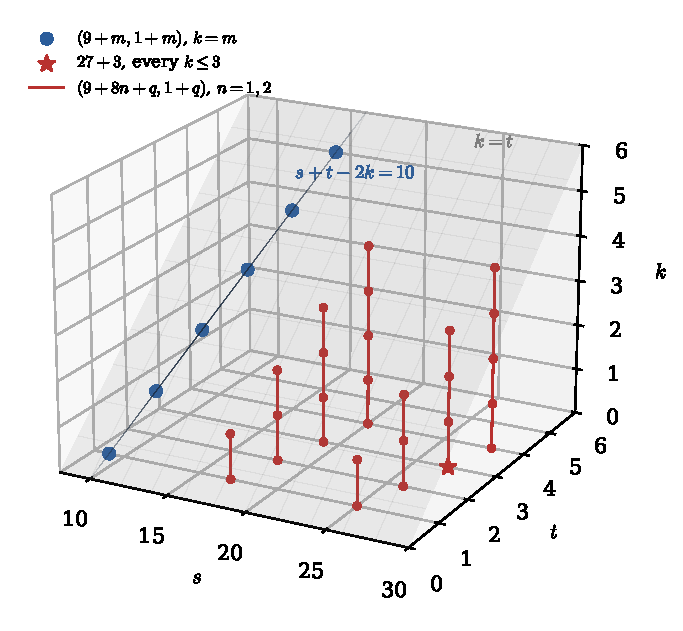
\includegraphics[width=0.78\textwidth]{figures/fig_signatures.pdf}
\caption{Signatures $(s,t)$ and numbers $k$ of null vectors. Blue points: Nishino's signatures $(9+m)+(1+m)$ with $k=m$, on the plane $s+t-2k=10$ (blue). Red segments: the signatures $(9+8n+q)+(1+q)$ of the families~\eqref{eq:families} for $n=1,2$ and $q=0,1,2,3$, with every $k\le t$; the star marks $27+3$. The grey surface is the wall $k=t$, beyond which real null frames do not exist. No red point reaches the blue plane.}
\label{fig:signatures}
\end{figure}

\begin{figure}[t]
\centering
\begin{adjustbox}{max width=\linewidth}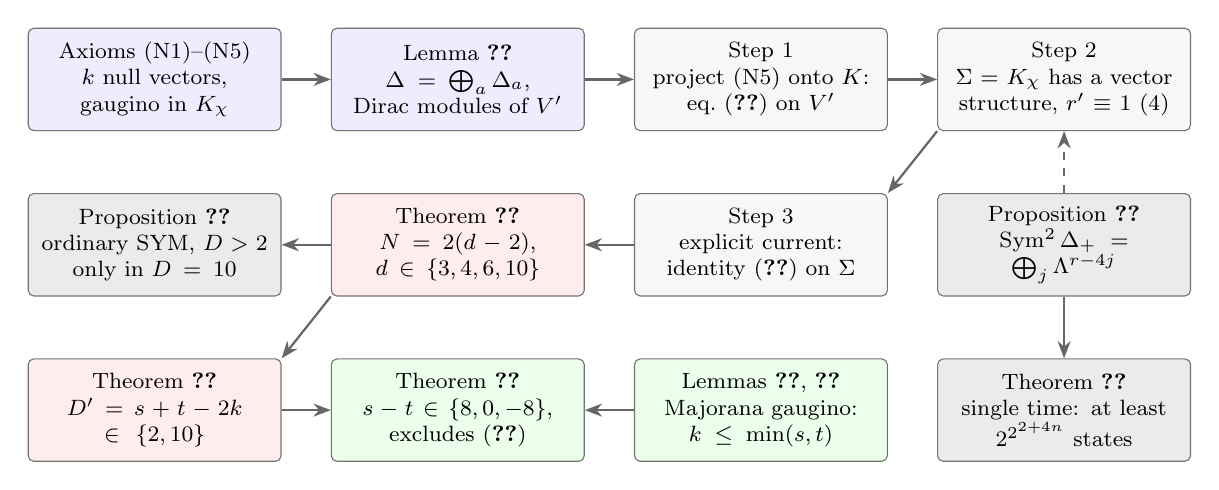
\begin{tikzpicture}[
  box/.style={draw=black!55,rounded corners=2pt,fill=#1,align=center,font=\footnotesize,inner sep=3pt,text width=3.0cm,minimum height=1.3cm},
  box/.default=black!3,
  arr/.style={-{Stealth[length=2.2mm]},thick,black!60}]
  \def\dx{3.85}
  \node[box=blue!7]  (ax)   at (0,0)        {Axioms (N1)--(N5)\\ $k$ null vectors,\\ gaugino in $K_\chi$};
  \node[box=blue!7]  (osc)  at (\dx,0)      {Lemma~\ref{lem:fock}\\ $\Delta=\bigoplus_a\Delta_a$,\\ Dirac modules of $V'$};
  \node[box]         (s1)   at (2*\dx,0)    {Step~1\\ project (N5) onto $K$:\\ eq.~\eqref{eq:proj1} on $V'$};
  \node[box]         (s2)   at (3*\dx,0)    {Step~2\\ $\Sigma=K_\chi$ has a vector\\ structure, $r'\equiv1$ (4)};
  \node[box=black!8] (std)  at (0,-2.1)     {Proposition~\ref{prop:standard}\\ ordinary SYM, $D>2$\\ only in $D=10$};
  \node[box=red!7]   (vec)  at (\dx,-2.1)   {Theorem~\ref{thm:vector}\\ $N=2(d-2)$,\\ $d\in\{3,4,6,10\}$};
  \node[box]         (s3)   at (2*\dx,-2.1) {Step~3\\ explicit current:\\ identity~\eqref{eq:R} on $\Sigma$};
  \node[box=black!8] (sym)  at (3*\dx,-2.1) {Proposition~\ref{prop:sym2}\\ $\Sym^2\Delta_+=$\\ $\bigoplus_j\Lambda^{r-4j}$};
  \node[box=red!7]   (red)  at (0,-4.2)     {Theorem~\ref{thm:reduction}\\ $D'=s+t-2k$\\ $\in\{2,10\}$};
  \node[box=green!8] (main) at (\dx,-4.2)   {Theorem~\ref{thm:main}\\ $s-t\in\{8,0,-8\}$,\\ excludes~\eqref{eq:families}};
  \node[box=green!8] (witt) at (2*\dx,-4.2) {Lemmas~\ref{lem:witt}, \ref{lem:reality}\\ Majorana gaugino:\\ $k\le\min(s,t)$};
  \node[box=black!8] (one)  at (3*\dx,-4.2) {Theorem~\ref{thm:singletime}\\ single time: at least\\ $2^{2^{2+4n}}$ states};
  \draw[arr] (ax)--(osc);
  \draw[arr] (osc)--(s1);
  \draw[arr] (s1)--(s2);
  \draw[arr] (s2.south west)--(s3.north east);
  \draw[arr,dashed] (sym)--(s2);
  \draw[arr] (s3)--(vec);
  \draw[arr] (vec)--(std);
  \draw[arr] (vec.south west)--(red.north east);
  \draw[arr] (red)--(main);
  \draw[arr] (witt)--(main);
  \draw[arr] (sym)--(one);
\end{tikzpicture}\end{adjustbox}
\caption{The logical structure of the paper. The axioms pass through the oscillator decomposition and Steps~1--3 to the identity~\eqref{eq:R} on the residual spinors; Theorem~\ref{thm:vector} turns that identity into $D'\in\{2,10\}$, and the bound on the number of null vectors converts this into a condition on $s-t$. Proposition~\ref{prop:sym2} enters Step~2 (dashed) and the single-time theorem. Proposition~\ref{prop:standard} is the case without null vectors.}
\label{fig:proofmap}
\end{figure}

\section{Spinors in signature \texorpdfstring{$(s,t)$}{(s,t)}}
\label{sec:spinors}

\subsection{Conventions}

Let $V=\bR^{s,t}$ with metric
\[
\eta=\operatorname{diag}(+1,\dots,+1,-1,\dots,-1),
\]
with $s$ plus signs and $t$ minus signs, and $D=s+t$. Except in Remark~\ref{rem:odd} we take $D=2r$ with $r\ge1$. The Clifford relations are $\gamma^\mu\gamma^\nu+\gamma^\nu\gamma^\mu=2\eta^{\mu\nu}$. The Dirac module $\Delta$ of the complex Clifford algebra $\Cl(V_\bC)$ has dimension $2^r$ and splits into the Weyl modules $\Delta_\pm$ of dimension $2^{r-1}$, the eigenspaces of the chirality operator $\Gamma_*$, normalized so that $\Gamma_*^2=1$. For a vector $u$ we write $\usl=u_\mu\gamma^\mu$, and $\gamma^{\mu_1\cdots\mu_p}$ is the antisymmetrized product of unit weight, so that $\gamma^{\mu_1\cdots\mu_p}=\allowbreak\gamma^{\mu_1}\cdots\gamma^{\mu_p}$ when the indices are distinct and the basis is orthonormal.

There is a nondegenerate bilinear form $B$ on $\Delta$, unique up to a factor once a sign $\theta=\pm1$ is chosen, such that
\begin{equation}
\label{eq:Bsym}
B(\gamma^\mu\psi,\chi)=\theta\,B(\psi,\gamma^\mu\chi),\qquad B(\psi,\chi)=\epsilon_B\,B(\chi,\psi),
\end{equation}
with $\epsilon_B=\pm1$ determined by $r$ and $\theta$~\cite{Deligne1999,VanProeyen1999,DAuriaFerraraLledoVaradarajan2001}. We write $\bar\psi\chi=B(\psi,\chi)$ and $\bar\psi\gamma^{\mu_1\cdots\mu_p}\chi=B(\psi,\gamma^{\mu_1\cdots\mu_p}\chi)$. The form $B$ pairs $\Delta_+$ with $\Delta_+$ when $r$ is even and with $\Delta_-$ when $r$ is odd.

A real structure on $\Delta$ is an antilinear map $C:\Delta\to\Delta$ with $C^2=1$ that commutes with every $\gamma^\mu$. It exists exactly when $s-t\equiv0,1,2\pmod 8$, and it preserves $\Delta_\pm$ exactly when $s-t\equiv0\pmod 8$~\cite{LawsonMichelsohn1989,Deligne1999,VanProeyen1999}. A Majorana spinor is a spinor with $C\psi=\psi$. Majorana--Weyl spinors, which are the spinors of all the theories in this paper, therefore exist if and only if $s-t\equiv 0\pmod 8$, and every signature in~\eqref{eq:families} and in Nishino's list has this property.

\subsection{The symmetric square of a Weyl spinor}

The anticommutator of two supercharges in the Weyl module $\Delta_+$ is a symmetric element of $\Delta_+\otimes\Delta_+$, so the superalgebras that can be written down in signature $(s,t)$ are classified by the decomposition of $\Sym^2\Delta_+$~\cite{vanHoltenVanProeyen1982,DAuriaFerraraLledoVaradarajan2001}. We write $\Lambda^p=\Lambda^pV_\bC$, and $\Lambda^r$ stands for the half $\Lambda^r_+$ of the middle-dimensional forms selected by $\Delta_+$.

\begin{proposition}
\label{prop:sym2}
For $D=2r$,
\begin{equation}
\label{eq:sym2}
\Sym^2\Delta_+\cong\bigoplus_{j\ge0,\ r-4j\ge0}\Lambda^{r-4j},\qquad \Lambda^2\Delta_+\cong\bigoplus_{j\ge0,\ r-2-4j\ge0}\Lambda^{r-2-4j}.
\end{equation}
In particular $\Lambda^1\subset\Sym^2\Delta_+$ if and only if $r\equiv1\pmod 4$, that is $D\equiv2\pmod 8$, and $\Lambda^1\subset\Lambda^2\Delta_+$ if and only if $r\equiv3\pmod 4$.
\end{proposition}

\begin{proof}
The forms $(\psi,\chi)\mapsto\bar\psi\gamma^{\mu_1\cdots\mu_p}\chi$ restricted to $\Delta_+\times\Delta_+$ vanish unless $p\equiv r\pmod 2$, and those with $p\equiv r\pmod 2$, $0\le p\le r$, give an isomorphism $\Delta_+\otimes\Delta_+\cong\bigoplus_{p}\Lambda^p$~\cite{Deligne1999,VanProeyen1999}. (As a check, $\sum_{p\equiv r\,(2),\,p<r}\binom{2r}{p}+\frac12\binom{2r}{r}=2^{2r-2}=(\dim\Delta_+)^2$.) It remains to decide which summands are symmetric. By~\eqref{eq:Bsym},
\[
\bar\psi\gamma^{\mu_1\cdots\mu_p}\chi=\theta^p\,B(\gamma^{\mu_p\cdots\mu_1}\psi,\chi)=\theta^p(-1)^{p(p-1)/2}\epsilon_B\;\bar\chi\gamma^{\mu_1\cdots\mu_p}\psi ,
\]
so the $p$-th form has symmetry $\sigma_p=\epsilon_B\theta^p(-1)^{p(p-1)/2}$, and $\sigma_{p+2}/\sigma_p=\theta^2(-1)^{2p+1}=-1$. The symmetric summands are therefore either those with $p\equiv r\pmod 4$ or those with $p\equiv r-2\pmod 4$. Using $\binom{2r}{p}=\binom{2r}{2r-p}$ and summing over the fourth roots of unity, the first set has total dimension
\[
\frac12\sum_{\substack{0\le p\le 2r\\ p\equiv r\,(4)}}\binom{2r}{p}=\frac18\sum_{\omega^4=1}\omega^{-r}(1+\omega)^{2r}=\frac18\bigl(2^{2r}+2^{r+1}\bigr)=2^{2r-3}+2^{r-2},
\]
because $i^{-r}(1+i)^{2r}=i^{r}(1-i)^{2r}=2^r$ and the term with $\omega=-1$ vanishes. This is $N(N+1)/2$ for $N=2^{r-1}$, while the second set has dimension $N(N-1)/2$. Hence the symmetric summands are those with $p\equiv r\pmod 4$.
\end{proof}

Appendix~\ref{app:tables} lists the decomposition for the families~\eqref{eq:families}. For $(9+8n)+1$ one has $r=5+4n$, and $\Sym^2\Delta_+$ consists of the forms of degrees $1,5,\dots,5+4n$; for $(10+8n)+2$ the degrees are $2,6,\dots,6+4n$; for $(11+8n)+3$ they are $3,7,\dots,7+4n$; and for $(12+8n)+4$ they are $0,4,\dots,8+4n$. These are exactly the right-hand sides of eqs.~(3.5)--(3.8) of Ref.~\cite{RiosMarraniChester2019}. The superalgebras proposed there are therefore maximal central supertranslation algebras: the anticommutator of two supercharges is an arbitrary element of $\Sym^2\Delta_+$, with a central charge for every summand. Such an algebra exists for every Weyl spinor in every signature, and its existence alone does not establish a field-theoretic realization.\footnote{For $27+3$ one has $r=15$ and $\Sym^2\Delta_+=\Lambda^{15}_+\oplus\Lambda^{11}\oplus\Lambda^7\oplus\Lambda^3$, of dimension $77\,558\,760+54\,627\,300+2\,035\,800+4\,060=134\,225\,920=2^{13}(2^{14}+1)$. These are the $3$-, $7$-, $11$- and $15$-form charges of eq.~(2.1) of Ref.~\cite{RiosMarraniChester2020}.} It contains the momentum only for $r\equiv1\pmod4$.

\subsection{Isotropic subspaces}

A subspace $U$ of $V$ or of $V_\bC$ is totally isotropic if $u\cdot u'=0$ for all $u,u'\in U$.

\begin{lemma}
\label{lem:witt}
A real totally isotropic subspace $U\subset\bR^{s,t}$ has $\dim U\le\min(s,t)$, and the bound is attained.\footnote{The number $\min(s,t)$ is the Witt index of $\eta$~\cite{Witt1937,Lam2005}.}
\end{lemma}

\begin{proof}
Write $V=V_+\oplus V_-$ with $V_+$ positive definite of dimension $s$ and $V_-$ negative definite of dimension $t$. If $u\in U\cap V_-$, then $u\cdot u=0$ forces $u=0$, so the projection $U\to V_+$ is injective and $\dim U\le s$. Exchanging the roles gives $\dim U\le t$. With orthonormal bases $e_1,\dots,e_s$ of $V_+$ and $f_1,\dots,f_t$ of $V_-$, the vectors $e_i+f_i$, $i\le\min(s,t)$, span a totally isotropic subspace of dimension $\min(s,t)$.
\end{proof}

The next lemma says that a Majorana spinor cannot distinguish a complex null vector from its complex conjugate.

\begin{lemma}
\label{lem:reality}
Let $s-t\equiv0,1,2\pmod 8$ and let $\lambda\ne0$ be a Majorana spinor. The set $U_\lambda=\{u\in V_\bC:\usl\lambda=0\}$ is a complex totally isotropic subspace invariant under complex conjugation. Hence $U_\lambda=U_\bR\otimes\bC$ with $U_\bR\subset V$ real and totally isotropic, and $\dim_\bC U_\lambda\le\min(s,t)$.
\end{lemma}

\begin{proof}
If $\usl\lambda=0$ and $\usl'\lambda=0$, then $2(u\cdot u')\lambda=(\usl\usl'+\usl'\usl)\lambda=0$, so $u\cdot u'=0$. Since $C$ is antilinear and commutes with the $\gamma^\mu$, $C(\usl\lambda)=\bar u_\mu\gamma^\mu C\lambda=\bar{\usl}\lambda$, so $\usl\lambda=0$ implies $\bar{\usl}\lambda=0$. A conjugation-invariant complex subspace is the complexification of its real points, and the real points of a totally isotropic subspace form a totally isotropic subspace of $V$. Lemma~\ref{lem:witt} finishes the proof.
\end{proof}

Figure~\ref{fig:lightcone} illustrates the lemma in $\bR^{2,1}$, where $\min(s,t)=1$: two independent real null vectors are never orthogonal.

\begin{figure}[t]
\centering
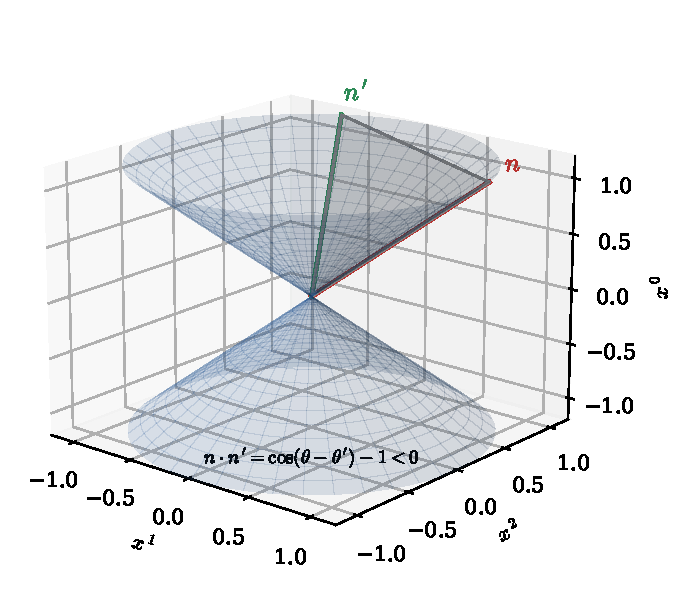
\includegraphics[width=0.56\textwidth]{figures/fig_lightcone.pdf}
\caption{The light cone of $\bR^{2,1}$. Two independent real null vectors $n=(\cos\theta,\sin\theta,1)$ and $n'=(\cos\theta',\sin\theta',1)$ satisfy $n\cdot n'=\cos(\theta-\theta')-1<0$, so the plane they span (grey) is not isotropic. In $\bR^{s,t}$ the largest isotropic subspaces have dimension $\min(s,t)$ (Lemma~\ref{lem:witt}).}
\label{fig:lightcone}
\end{figure}

\section{Vector structures and the cubic identity}
\label{sec:vector}

Every condition on cubic fermion terms that appears in this paper is a statement about the following structure.

\begin{definition}
\label{def:vector}
Let $W$ be a complex vector space of dimension $d$ with a nondegenerate symmetric bilinear form $\eta$, and let $\Sigma$ be a complex vector space of dimension $N\ge1$ with dual $\Sigma^*$. A \emph{vector structure} on $\Sigma$ is a pair of linear maps, $\gamma$ from $W$ to the symmetric maps $\Sigma\to\Sigma^*$ and $\tilde\gamma$ from $W$ to the maps $\Sigma^*\to\Sigma$, such that in a basis of $W$
\begin{equation}
\label{eq:clifford}
\tilde\gamma^\mu\gamma^\nu+\tilde\gamma^\nu\gamma^\mu=2\eta^{\mu\nu}\,1_\Sigma,\qquad \gamma^\mu\tilde\gamma^\nu+\gamma^\nu\tilde\gamma^\mu=2\eta^{\mu\nu}\,1_{\Sigma^*}.
\end{equation}
In a basis $e_\alpha$ of $\Sigma$ we write $\gamma^\mu_{\alpha\beta}$ and $\tilde\gamma^{\mu\,\alpha\beta}$ for the matrix entries; $\gamma^\mu_{\alpha\beta}=\gamma^\mu_{\beta\alpha}$.
\end{definition}

The standard example is $\Sigma=\Delta_+$ in $D=2r$ with $r$ odd, $\Sigma^*\cong\Delta_-$ through $B$, $\gamma^\mu_{\alpha\beta}=B(e_\alpha,\gamma^\mu e_\beta)$, and $\tilde\gamma^\mu$ the Clifford action $\Delta_-\to\Delta_+$; by Proposition~\ref{prop:sym2} the forms are symmetric when $r\equiv1\pmod4$. In ten dimensions these are the familiar $16\times16$ matrices $\sigma^\mu_{\alpha\beta}$ and $\bar\sigma^{\mu\,\alpha\beta}$~\cite{FreedmanVanProeyen2012}.

\begin{lemma}
\label{lem:traces}
Let $(\Sigma,\gamma,\tilde\gamma)$ be a vector structure with $d\ge3$. Then
\begin{enumerate}[label=(\alph*)]
\item each $\tilde\gamma^\mu$ is symmetric, and in an orthonormal basis $\tilde\gamma^\mu=\eta^{\mu\mu}(\gamma^\mu)^{-1}$ (no sum);
\item $\gamma_\mu\tilde\gamma^\mu=d\,1_{\Sigma^*}$ and $\gamma_\mu\tilde\gamma^\nu\gamma^\mu=-(d-2)\gamma^\nu$;
\item $\tr_{\Sigma^*}(\gamma^\mu\tilde\gamma^\nu)=\gamma^\mu_{\alpha\beta}\tilde\gamma^{\nu\,\beta\alpha}=N\eta^{\mu\nu}$.
\end{enumerate}
\end{lemma}

\begin{proof}
(a) Setting $\mu=\nu$ in~\eqref{eq:clifford} gives $\gamma^\mu\tilde\gamma^\mu=\eta^{\mu\mu}1_{\Sigma^*}$ and $\tilde\gamma^\mu\gamma^\mu=\eta^{\mu\mu}1_\Sigma$, and the inverse of a symmetric map is symmetric. (b) Contracting the second relation in~\eqref{eq:clifford} gives the first identity, and then $\gamma_\mu\tilde\gamma^\nu\gamma^\mu=\gamma_\mu(2\eta^{\nu\mu}-\tilde\gamma^\mu\gamma^\nu)=2\gamma^\nu-d\gamma^\nu$. (c) On $\Sigma\oplus\Sigma^*$ the operators $\Gamma^\mu=\begin{psmallmatrix}0&\tilde\gamma^\mu\\ \gamma^\mu&0\end{psmallmatrix}$ obey $\Gamma^\mu\Gamma^\nu+\Gamma^\nu\Gamma^\mu=2\eta^{\mu\nu}$, and $\Gamma_*=\operatorname{diag}(1,-1)$ anticommutes with every $\Gamma^\mu$. In an orthonormal basis take $\mu\ne\nu$ and choose $\rho\notin\{\mu,\nu\}$, which is possible because $d\ge3$. The invertible operator $\Gamma^\rho$ commutes with $\Gamma^\mu\Gamma^\nu$ and anticommutes with $\Gamma_*\Gamma^\mu\Gamma^\nu$, so $\tr(\Gamma_*\Gamma^\mu\Gamma^\nu)=0$; and $\tr(\Gamma^\mu\Gamma^\nu)=-\tr(\Gamma^\nu\Gamma^\mu)=0$. The restriction of $\Gamma^\mu\Gamma^\nu=\operatorname{diag}(\tilde\gamma^\mu\gamma^\nu,\gamma^\mu\tilde\gamma^\nu)$ to $\Sigma^*$ is $\gamma^\mu\tilde\gamma^\nu$, and its trace $\frac12\tr\bigl((1-\Gamma_*)\Gamma^\mu\Gamma^\nu\bigr)$ therefore vanishes for $\mu\ne\nu$. For $\mu=\nu$ it is $N\eta^{\mu\mu}$ by (a).
\end{proof}

The condition that absorption of cubic terms will produce is the following. For a constant $j\in\bC$ consider
\begin{equation}
\label{eq:R}
\tfrac12\bigl(\gamma^\mu_{\alpha\beta}\gamma_{\mu\,\gamma\delta}+\gamma^\mu_{\alpha\gamma}\gamma_{\mu\,\beta\delta}\bigr)=j\,\gamma^\sigma_{\alpha\delta}\gamma_{\sigma\,\beta\gamma}\qquad\text{for all }\alpha,\beta,\gamma,\delta.
\end{equation}
For $j=-\frac12$ this is the identity~\eqref{eq:star}.

\begin{theorem}
\label{thm:vector}
Let $(\Sigma,\gamma,\tilde\gamma)$ be a vector structure with $d\ge3$, and suppose that~\eqref{eq:R} holds for some $j\in\bC$. Then
\begin{equation}
\label{eq:N}
N=2(d-2),\qquad j=-\tfrac12,
\end{equation}
so the identity is~\eqref{eq:star}. Moreover $N$ is divisible by $2^{\lceil d/2\rceil-1}$, and therefore $(d,N)\in\{(3,2),(4,4),(6,8),(10,16)\}$.
\end{theorem}

\begin{proof}
Contract~\eqref{eq:R} with $\tilde\gamma^{\nu\,\delta\gamma}$, which is symmetric by Lemma~\ref{lem:traces}(a), and sum over $\gamma,\delta$. Inside the bracket on the left, the first term gives $\gamma^\mu_{\alpha\beta}\tr(\gamma_\mu\tilde\gamma^\nu)=N\gamma^\nu_{\alpha\beta}$ and the second gives $(\gamma^\mu\tilde\gamma^\nu\gamma_\mu)_{\alpha\beta}=-(d-2)\gamma^\nu_{\alpha\beta}$, by Lemma~\ref{lem:traces}(b),(c). The right-hand side gives $j(\gamma^\sigma\tilde\gamma^\nu\gamma_\sigma)_{\alpha\beta}=-j(d-2)\gamma^\nu_{\alpha\beta}$. Since $\gamma^\nu\ne0$,
\begin{equation}
\label{eq:contr1}
N-(d-2)=-2j(d-2).
\end{equation}
Next contract with $\tilde\gamma^{\nu\,\beta\gamma}$ and sum over $\beta,\gamma$. Both terms in the bracket give $(\gamma^\mu\tilde\gamma^\nu\gamma_\mu)_{\alpha\delta}=-(d-2)\gamma^\nu_{\alpha\delta}$, and the right-hand side gives $j\gamma^\sigma_{\alpha\delta}\tr(\gamma_\sigma\tilde\gamma^\nu)=jN\gamma^\nu_{\alpha\delta}$, so
\begin{equation}
\label{eq:contr2}
jN=-(d-2).
\end{equation}
Substituting $j=-(d-2)/N$ into~\eqref{eq:contr1} gives $N^2-(d-2)N-2(d-2)^2=0$, that is $(N-2(d-2))(N+d-2)=0$. As $N+d-2>0$, we get $N=2(d-2)$ and $j=-\frac12$.

For the divisibility, the operators $\Gamma^\mu$ and $\Gamma_*$ of the proof of Lemma~\ref{lem:traces}(c) make $\Sigma\oplus\Sigma^*$ a module over the complex Clifford algebra on $d+1$ generators. This algebra is semisimple and its irreducible modules have dimension $2^{\lfloor(d+1)/2\rfloor}=2^{\lceil d/2\rceil}$, so $2^{\lceil d/2\rceil}$ divides $2N=4(d-2)$. For $d=5,7,8,9$ it does not, and for $d\ge11$ one has $4(d-2)<2^{\lceil d/2\rceil}$. This leaves $d=3,4,6,10$.
\end{proof}

\begin{remark}
\label{rem:division}
The four solutions are the Majorana spinors of three and four dimensions, the Weyl spinors of six (with their $Sp(1)$ doublet) and the Majorana--Weyl spinors of ten, and in each case~\eqref{eq:star} holds~\cite{KugoTownsend1983,Evans1988,BaezHuerta2010}. Theorem~\ref{thm:vector} is a converse that makes no reference to division algebras and allows a general constant $j$: the dimension count alone fixes both $N$ and $j$. The constant $j$ is left free because absorbing the cubic terms into a modified field equation, the mechanism of Nishino's construction, produces~\eqref{eq:R} with a constant that is not known in advance (Sec.~\ref{sec:null}). Figure~\ref{fig:spinorcount} compares $2(d-2)$ with the smallest admissible $N$.
\end{remark}

\begin{figure}[t]
\centering
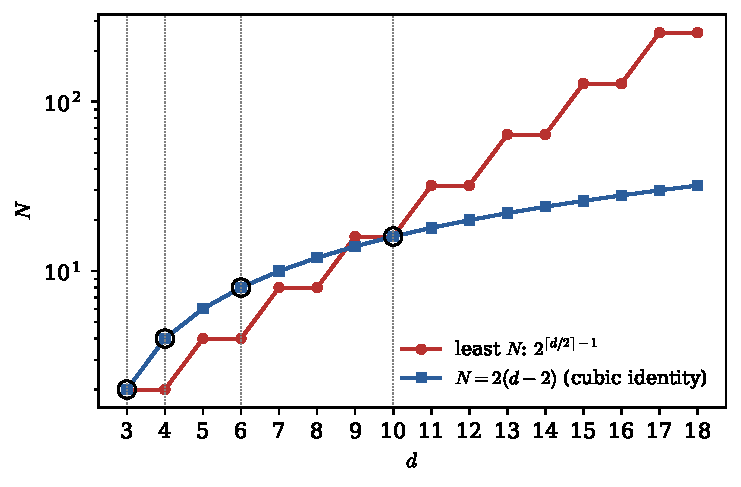
\includegraphics[width=0.64\textwidth]{figures/fig_spinorcount.pdf}
\caption{The spinor dimension $N=2(d-2)$ forced by the cubic identity (blue) against the smallest dimension $2^{\lceil d/2\rceil-1}$ that a vector structure can have (red). A solution requires the blue value to be a multiple of the red one. This happens for $d=3,4,6,10$ (circles) and never again, because the red curve grows exponentially.}
\label{fig:spinorcount}
\end{figure}

\section{Ordinary super Yang--Mills theory}
\label{sec:standard}

Before turning to null projections we record what Theorem~\ref{thm:vector} gives without them. Let the gauge algebra $\ad$ be a compact non-abelian Lie algebra with structure constants $f^{IJK}$, totally antisymmetric in an orthonormal basis. Let the gaugino $\lambda^I$ and the parameter $\epsilon$ be Grassmann-odd Weyl spinors in $\Delta_+$ (Majorana--Weyl when $s-t\equiv0\pmod8$), and consider
\begin{equation}
\label{eq:lagr}
\mathcal L=-\tfrac14F^I_{\mu\nu}F^{I\mu\nu}+\tfrac c2\,\bar\lambda^I\gamma^\mu D_\mu\lambda^I,\qquad \delta A^I_\mu=a\,\bar\epsilon\gamma_\mu\lambda^I,\qquad \delta\lambda^I=b\,\gamma^{\mu\nu}F^I_{\mu\nu}\epsilon ,
\end{equation}
with $D_\mu\lambda^I=\partial_\mu\lambda^I+gf^{IJK}A^J_\mu\lambda^K$ and nonzero constants $a,b,c,g$.

\begin{proposition}
\label{prop:standard}
Assume $D>2$ and that the gaugino term in~\eqref{eq:lagr} is a nondegenerate kinetic term, rather than zero or a total derivative. If $\delta\mathcal L$ is a total derivative, then the forms $\gamma^\mu_{\alpha\beta}=B(e_\alpha,\gamma^\mu e_\beta)$ on $\Delta_+$ define a vector structure satisfying~\eqref{eq:star}. Consequently $D=10$, and with Majorana--Weyl spinors the signature is $(9,1)$, $(5,5)$ or $(1,9)$.
\end{proposition}

\begin{proof}
The kinetic term is nonzero only if $B$ pairs $\Delta_+$ with $\gamma^\mu\Delta_+=\Delta_-$, that is for $r$ odd, and it is not a total derivative only if the form $\gamma^\mu_{\alpha\beta}$ is symmetric: for Grassmann-odd $\lambda$ and antisymmetric $G$, $\lambda^\alpha G_{\alpha\beta}\partial\lambda^\beta=\frac12\partial(\lambda^\alpha G_{\alpha\beta}\lambda^\beta)$. With $\Sigma=\Delta_+$, $\Sigma^*\cong\Delta_-$ and $\tilde\gamma^\mu$ the Clifford action $\Delta_-\to\Delta_+$, the relations~\eqref{eq:clifford} are those of $\Cl(V)$, so $(\Delta_+,\gamma,\tilde\gamma)$ is a vector structure with $d=D$ and $N=2^{r-1}$.

The terms of $\delta\mathcal L$ cubic in $\lambda$ come only from $\delta A$ inside the covariant derivative, since $\delta\lambda$ is linear in $F$ and $\delta F$ is linear in $\lambda$. They are
\begin{equation}
\label{eq:cubic}
\begin{aligned}\tfrac{c}{2}\,ag\,f^{IJK}\,(\bar\lambda^I\gamma^\mu\lambda^K)(\bar\epsilon\gamma_\mu\lambda^J)&=\pm\tfrac{c}{2}\,ag\;\gamma^\mu_{\alpha\gamma}\gamma_{\mu\,\delta\beta}\,\epsilon^\delta\,T^{\alpha\beta\gamma},\\ T^{\alpha\beta\gamma}&=f^{IJK}\lambda^{I\alpha}\lambda^{J\beta}\lambda^{K\gamma}.\end{aligned}
\end{equation}
where the sign depends only on the ordering convention for Grassmann variables. They contain no derivative, so they must vanish. The tensor $T$ is totally symmetric: exchanging two of its indices and relabelling the gauge indices produces one sign from $f$ and one from the anticommuting $\lambda$. It spans $\Sym^3\Sigma$. Indeed $\ad$ contains a subalgebra $\mathfrak{su}(2)$, and for $\lambda$ with values in it $T^{\alpha\beta\gamma}c_{\alpha\beta\gamma}=6c_{\alpha\beta\gamma}\lambda^{1\alpha}\lambda^{2\beta}\lambda^{3\gamma}$ for every symmetric $c$, after normalizing $f^{123}=1$. Since the monomials $\lambda^{1\alpha}\lambda^{2\beta}\lambda^{3\gamma}$ are linearly independent, only $c=0$ annihilates every $T$. Hence, for every $\delta$, the part of $\gamma^\mu_{\alpha\gamma}\gamma_{\mu\,\delta\beta}$ symmetric in $\alpha,\beta,\gamma$ vanishes. Because each factor is symmetric in its own pair of indices, that symmetrization is one third of the sum over the three ways of pairing $\delta$ with $\alpha$, $\beta$ or $\gamma$, which is~\eqref{eq:star}. Theorem~\ref{thm:vector} with $N=2^{r-1}$ and $d=2r$ gives $2^{r-1}=4(r-1)$, whose only solution with $r\ge2$ is $r=5$. Majorana--Weyl spinors in $D=10$ require $s-t\in\{8,0,-8\}$.
\end{proof}

The proposition is the familiar statement that ten is the largest dimension of super Yang--Mills theory~\cite{BrinkSchwarzScherk1977}, obtained here from the dimension count of Theorem~\ref{thm:vector} rather than from an explicit Fierz rearrangement. For $D>2$, changing the signature does not evade this conventional nondegenerate-kinetic-term ansatz, because the proof uses only $D$. The degenerate two-dimensional case is not covered by the proposition. The higher-dimensional constructions examined here therefore constrain the gaugino.

\section{Null-projected super Yang--Mills theories}
\label{sec:null}

\subsection{Null frames as fermionic oscillators}

\begin{definition}
\label{def:frame}
A \emph{null frame of rank $k$} is a set of vectors $n_1,\dots,n_k,\allowbreak m_1,\dots,m_k\in V_\bC$ with
\begin{equation}
\label{eq:frame}
n_i\cdot n_j=0,\qquad m_i\cdot m_j=0,\qquad n_i\cdot m_j=\delta_{ij}.
\end{equation}
It is \emph{real} if all the vectors lie in $V$. Its \emph{residual space} is the orthogonal complement $V'$ of $\Span(n_i,m_i)$, of dimension $D'=D-2k$, and we set $v=n_1\wedge\cdots\wedge n_k$.
\end{definition}

The span of the $n_i$ and $m_i$ is a sum of $k$ hyperbolic planes, so for a real frame $V'$ is real of signature $(s-k,t-k)$. By Lemma~\ref{lem:witt}, a real null frame of rank $k$ exists exactly when $k\le\min(s,t)$. In Nishino's notation $n_i=n_{(i)}$ and $m_i=m_{(i)}$; his signatures $(9+m)+(1+m)$ carry real frames of rank $m$ with residual space $\bR^{9,1}$.

The relations~\eqref{eq:frame} say that the operators
\begin{equation}
\label{eq:osc}
b_i=\tfrac{1}{\sqrt2}\msl_i,\qquad b_i^\dagger=\tfrac{1}{\sqrt2}\nsl_i
\end{equation}
obey the canonical anticommutation relations $\{b_i,b_j^\dagger\}=\delta_{ij}$, $\{b_i,b_j\}=\{b_i^\dagger,b_j^\dagger\}=0$. (The dagger is notation; no adjoint is implied.) The number operators
\begin{equation}
\label{eq:proj}
\Pup_i=b_i^\dagger b_i=\tfrac12\nsl_i\msl_i,\qquad \Pdn_i=b_ib_i^\dagger=\tfrac12\msl_i\nsl_i=1-\Pup_i
\end{equation}
are Nishino's projectors~\cite{Nishino1998}, and they commute with each other. For $a\in\{0,1\}^k$ let $\Delta_a$ be the joint eigenspace on which $\Pup_i=a_i$; mode $i$ is occupied in $\Delta_a$ if $a_i=1$. Write $\mathbf 1=(1,\dots,1)$, $\mathbf 0=(0,\dots,0)$, $\bar a=\mathbf 1-a$, and $e_i$ for the $i$-th unit vector of $\{0,1\}^k$. For vectors of $V'$ we use primed indices, $\gamma^{\mu'}$.

\begin{lemma}
\label{lem:fock}
\begin{enumerate}[label=(\roman*)]
\item $\Delta=\bigoplus_a\Delta_a$. Each $\gamma^{\mu'}$ preserves every $\Delta_a$, and each $\Delta_a$ is a Dirac module of $\Cl(V'_\bC)$, of dimension $2^{r-k}$.
\item $\nsl_i$ maps $\Delta_a$ with $a_i=0$ isomorphically onto $\Delta_{a+e_i}$ and annihilates $\Delta_a$ with $a_i=1$; $\msl_i$ does the reverse. Hence
\begin{equation}
K:=\bigcap_i\ker\nsl_i=\Delta_{\mathbf 1},\qquad \Khat:=\bigcap_i\ker\msl_i=\Delta_{\mathbf 0}.
\end{equation}
\item $T=\nsl_1\nsl_2\cdots\nsl_k$ maps $\Khat$ isomorphically onto $K$, annihilates $\Delta_a$ for $a\ne\mathbf 0$, and satisfies $T\gamma^{\mu'}=(-1)^k\gamma^{\mu'}T$; in particular $T$ commutes with $\Spin(V')$.
\item $B(\Delta_a,\Delta_b)=0$ unless $b=\bar a$.
\item On each $\Delta_a$ the chirality $\Gamma_*$ equals $\pm(-1)^{|a|}\Gamma'_*$, where $\Gamma'_*$ is the chirality of $V'$, $|a|$ is the number of occupied modes, and the overall sign does not depend on $a$. Thus $\Delta_a\cap\Delta_+$ and $\Delta_a\cap\Delta_-$ are the two Weyl modules of $V'$.
\end{enumerate}
\end{lemma}

The proof is in Appendix~\ref{app:fock}. Figure~\ref{fig:cube} shows the case $k=3$. The kernel $K$ of all the $\nsl_i$ is the fully occupied corner, the kernel $\Khat$ of all the $\msl_i$ is the empty corner, $T$ climbs from one to the other, and $B$ pairs opposite corners.

\begin{figure}[t]
\centering
\begin{adjustbox}{max width=\linewidth}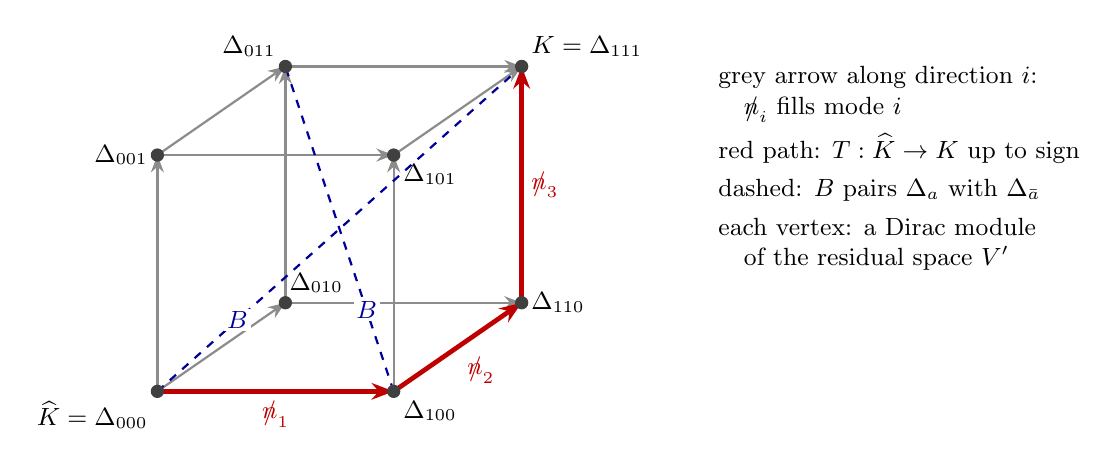
\begin{tikzpicture}[scale=1.25,
  vtx/.style={circle,fill=black!75,inner sep=1.7pt},
  edge/.style={-{Stealth[length=2.2mm]},thick,black!45},
  tpath/.style={-{Stealth[length=2.8mm]},line width=1.7pt,red!75!black},
  pair/.style={dashed,blue!60!black,thick},
  lab/.style={font=\small}]
  % oblique projection (x,y,z) -> (x+0.54y, z+0.38y), cube of side 2.4
  \coordinate (000) at (0,0);      \coordinate (100) at (2.4,0);
  \coordinate (001) at (0,2.4);    \coordinate (101) at (2.4,2.4);
  \coordinate (010) at (1.3,0.9); \coordinate (110) at (3.7,0.9);
  \coordinate (011) at (1.3,3.3); \coordinate (111) at (3.7,3.3);
  \draw[edge] (000)--(010); \draw[edge] (000)--(001);
  \draw[edge] (100)--(101);
  \draw[edge] (010)--(110); \draw[edge] (010)--(011);
  \draw[edge] (001)--(101); \draw[edge] (001)--(011);
  \draw[edge] (101)--(111); \draw[edge] (011)--(111);
  \draw[pair] (000)--(111);
  \draw[pair] (100)--(011);
  \draw[tpath] (000)--(100);
  \draw[tpath] (100)--(110);
  \draw[tpath] (110)--(111);
  \foreach \v in {000,100,010,001,110,101,011,111} \node[vtx] at (\v) {};
  \node[lab,below left] at (000) {$\Khat=\Delta_{000}$};
  \node[lab,below right] at (100) {$\Delta_{100}$};
  \node[lab,left] at (001) {$\Delta_{001}$};
  \node[lab,below right] at (101) {$\Delta_{101}$};
  \node[lab,above right,xshift=-2pt] at (010) {$\Delta_{010}$};
  \node[lab,right] at (110) {$\Delta_{110}$};
  \node[lab,above left] at (011) {$\Delta_{011}$};
  \node[lab,above right] at (111) {$K=\Delta_{111}$};
  \node[lab,red!75!black,below] at ($(000)!0.5!(100)$) {$\nsl_1$};
  \node[lab,red!75!black,below right] at ($(100)!0.5!(110)$) {$\nsl_2$};
  \node[lab,red!75!black,right] at ($(110)!0.5!(111)$) {$\nsl_3$};
  \node[lab,blue!60!black,fill=white,inner sep=1pt] at ($(000)!0.22!(111)$) {$B$};
  \node[lab,blue!60!black,fill=white,inner sep=1pt] at ($(100)!0.25!(011)$) {$B$};
  \node[align=left,anchor=north west,font=\small] at (5.6,3.4) {grey arrow along direction $i$:\\ \quad $\nsl_i$ fills mode $i$\\[3pt] red path: $T:\Khat\to K$ up to sign\\[3pt] dashed: $B$ pairs $\Delta_a$ with $\Delta_{\bar a}$\\[3pt] each vertex: a Dirac module\\ \quad of the residual space $V'$};
\end{tikzpicture}\end{adjustbox}
\caption{The decomposition of the Dirac module for a null frame of rank $k=3$. The vertices are the joint eigenspaces $\Delta_a$ of the number operators $\Pup_i$, each a Dirac module of the residual space $V'$. The gaugino lives in the fully occupied corner $K$; the supersymmetry parameters that act on the residual components of the gauge field live in the opposite corner $\Khat$.}
\label{fig:cube}
\end{figure}

\subsection{The axioms}

\begin{definition}
\label{def:npsym}
A \emph{null-projected super Yang--Mills theory of rank $k$} in signature $(s,t)$, $D=2r$, consists of a null frame of rank $k$, a compact non-abelian gauge algebra $\ad$, a gauge field $A^I_\mu$, a Grassmann-odd gaugino $\lambda^I$ and Grassmann-odd supersymmetry parameters $\epsilon$, subject to the following conditions.
\begin{enumerate}[label=(N\arabic*)]
\item\label{ax:N1} \emph{Constraint.} The complexified gaugino value space is the full corner $K_\chi=K\cap\Delta_\chi$ for a fixed chirality $\chi$; $\lambda^I$ takes values there, that is, $\nsl_i\lambda^I=0$ for all $i$. The parameter $\epsilon$ ranges over a Weyl module $\Delta_{\chi'}$.\footnote{As in Nishino's construction, $\epsilon$ is not constrained. The proof uses only the component of $\epsilon$ in $\Khat$, which by Lemma~\ref{lem:fock}(iv) is the only component that enters the residual components of $\delta A$. Any family of parameters whose $\Khat$-components form a nonzero $\Spin(V')$-invariant subspace leads to the same conclusions.}
\item\label{ax:N2} \emph{Transformations.} $\delta A^I_\mu=a\,\bar\epsilon\gamma_\mu\lambda^I$ with $a\ne0$, and $\delta\lambda^I=\Phi(F^I)\epsilon$ for a linear map $\Phi$ from two-forms to $\operatorname{End}\Delta$ that does not depend on $\lambda$. The covariant derivative is $D_\mu\lambda^I=\partial_\mu\lambda^I+gf^{IJK}A^J_\mu\lambda^K$ with $g\ne0$.
\item\label{ax:N3} \emph{Residual gauge field.} The components $\delta A^I_{\mu'}$ along $V'$ do not vanish identically.
\item\label{ax:N4} \emph{Closure.} The commutator of two supersymmetries contains the translation by
\begin{equation}
\label{eq:xi}
\xi^\mu=c\,\bar\epsilon_2\gamma^{\mu\nu_1\cdots\nu_k}\epsilon_1\,v_{\nu_1\cdots\nu_k},\qquad c\ne0,
\end{equation}
and its components $\xi^{\mu'}$ along $V'$ do not vanish identically. The displayed translation bracket is the coefficient in the supersymmetry anticommutator, so its matrix in the commuting spinor indices is symmetric. This graded symmetry is part of the closure requirement.
\item\label{ax:N5} \emph{Absorption.} For every $\lambda$ with values in $K_\chi\otimes\ad$ there are $J^I_\sigma$, depending on $\lambda$ but not on $\epsilon$, such that for every $\epsilon$ the part of $\delta(\gamma^\mu D_\mu\lambda^I)$ quadratic in $\lambda$ equals
\begin{equation}
\label{eq:absorb}
\gamma^{\sigma\nu_1\cdots\nu_k}\epsilon\;v_{\nu_1\cdots\nu_k}\,J^I_\sigma .
\end{equation}
\end{enumerate}
\end{definition}

Axiom~\ref{ax:N5} is what makes the theory consistent: a term of the form~\eqref{eq:absorb} is cancelled by a source term in the field equation of the gauge field, which becomes $D^\mu F_{\mu[\sigma}v_{\nu_1\cdots\nu_k]}\propto J_{[\sigma}v_{\nu_1\cdots\nu_k]}$. For $k=0$ the axiom says that the cubic terms have the form $\gamma^\sigma\epsilon J_\sigma$.

\begin{example}
\label{ex:nishino}
Nishino's theories~\cite{Nishino1998} in $(9+m)+(1+m)$ satisfy~\ref{ax:N1}--\ref{ax:N5} with $k=m$. His constraint~(2.12), the contraction of $v$ with $\gamma^\mu\lambda$, is equivalent to $\nsl_{(i)}\lambda=0$ for every $i$, and he rewrites it as $\lambda=\Pup\lambda$ in eq.~(2.22). The transformations~\ref{ax:N2} are his eq.~(2.3), with $\Phi(F)\epsilon=\frac14\gamma^{\mu\nu\rho_1\cdots\rho_m}\epsilon F_{\mu\nu}v_{\rho_1\cdots\rho_m}$, and the closure~\ref{ax:N4} is his eqs.~(2.16)--(2.18). Axiom~\ref{ax:N5} is his eq.~(2.29): the surviving cubic term is $\gamma^{[m+1]}\epsilon$ contracted with the bilinear $\bar\lambda^K\gamma_{[m+1]}\lambda^J$, and for gauginos in $K$ this $(m+1)$-form is the wedge product of $v$ with a residual vector (Lemma~\ref{lem:nullcurrent}), so the term has the form~\eqref{eq:absorb}; it is absorbed by the source in his field equation~(2.15).\footnote{Nishino writes $v_{[4n]}$ for the class $m=4n$ and treats $m=4n+1,4n+2,4n+3$ in the same way. We write $k$ for the number of null vectors in all cases.} The residual space is $\bR^{9,1}$, so $D'=10$.
\end{example}

The variation of the gaugino equation follows directly from the axioms.

\begin{lemma}
\label{lem:quadratic}
Under~\ref{ax:N2}, the part of $\delta(\gamma^\mu D_\mu\lambda^I)$ quadratic in $\lambda$ is $ag\,f^{IJK}\gamma^\mu\lambda^K\,(\bar\epsilon\gamma_\mu\lambda^J)$.
\end{lemma}

\begin{proof}
$\delta(D_\mu\lambda^I)=D_\mu(\delta\lambda^I)+gf^{IJK}\delta A^J_\mu\lambda^K$. The first term is independent of $\lambda$ because $\Phi$ is, and the second is $ag f^{IJK}(\bar\epsilon\gamma_\mu\lambda^J)\lambda^K$.
\end{proof}

\subsection{Reduction to the residual space}

\begin{theorem}
\label{thm:reduction}
In a null-projected super Yang--Mills theory of rank $k$ the residual dimension $D'=D-2k$ equals $10$ or $2$.
\end{theorem}

\begin{proof}
$D'$ is even, and $D'\ge1$ because~\ref{ax:N3} requires residual directions. Assume $D'\ge3$; we prove $D'=10$. The proof has three steps.

\emph{Step 1: projection onto the occupied corner.} Since $n_i\cdot m_j=\delta_{ij}$, the inverse metric decomposes as $\eta^{-1}=\eta'^{-1}+\sum_i(n_i\otimes m_i+m_i\otimes n_i)$, so
\begin{equation}
\label{eq:split}
\gamma^\mu\lambda\,(\bar\epsilon\gamma_\mu\lambda')=\gamma^{\mu'}\lambda\,(\bar\epsilon\gamma_{\mu'}\lambda')+\sum_i\bigl[\nsl_i\lambda\,(\bar\epsilon\msl_i\lambda')+\msl_i\lambda\,(\bar\epsilon\nsl_i\lambda')\bigr].
\end{equation}
For $\lambda,\lambda'\in K$ the bracket vanishes, because $\nsl_i$ annihilates $K$. By Lemma~\ref{lem:quadratic} the left-hand side of~\ref{ax:N5} is therefore
\begin{equation}
\label{eq:lhs}
ag\,f^{IJK}\gamma^{\mu'}\lambda^K(\bar\epsilon\gamma_{\mu'}\lambda^J),
\end{equation}
which lies in the occupied corner $\Delta_{\mathbf 1}$ because $\gamma^{\mu'}$ preserves every $\Delta_a$. On the right-hand side of~\eqref{eq:absorb}, write $\gamma(\omega)$ for the antisymmetrized product of gamma matrices attached to a $(k+1)$-vector $\omega$, normalized so that $\gamma(u_0\wedge\cdots\wedge u_k)=\usl_0\cdots\usl_k$ for mutually orthogonal $u_i$. Up to a nonzero factor, which we absorb into $J$, the right-hand side is $\gamma(J\wedge v)\epsilon$. Decompose $J=J'+\sum_i[(J\cdot n_i)\,m_i+(J\cdot m_i)\,n_i]$ with $J'\in V'_\bC$. Since $n_i\wedge v=0$, the vector $u'\in V'_\bC$ is orthogonal to all the $n_l$, and $m_i$ is orthogonal to all $n_l$ with $l\ne i$,
\begin{equation}
\label{eq:antisym}
\gamma(u'\wedge v)=\usl'\,T,\qquad \gamma(n_i\wedge v)=0,\qquad \gamma(m_i\wedge v)=\pm\Bigl(\prod_{l\ne i}\nsl_l\Bigr)(\Pdn_i-\Pup_i),
\end{equation}
where the last formula uses $\frac12(\msl_i\nsl_i-\nsl_i\msl_i)=\Pdn_i-\Pup_i$. Now take $\epsilon\in\Khat_{\chi'}=\Khat\cap\Delta_{\chi'}$. Then $\gamma^{\mu'}T\epsilon\in\Delta_{\mathbf 1}$, while $(\prod_{l\ne i}\nsl_l)(\Pdn_i-\Pup_i)\epsilon$ lies in $\Delta_{\mathbf 1-e_i}$, in which mode $i$ is empty. Applying the projection $\prod_i\Pup_i$ onto $\Delta_{\mathbf 1}$ to both sides of~\ref{ax:N5}, we obtain for all $\epsilon\in\Khat_{\chi'}$
\begin{equation}
\label{eq:proj1}
ag\,f^{IJK}\gamma^{\mu'}\lambda^K(\bar\epsilon\gamma_{\mu'}\lambda^J)=\gamma^{\mu'}T\epsilon\;J^I_{\mu'} .
\end{equation}

\emph{Step 2: the residual vector structure.} By Lemma~\ref{lem:fock}(iii), $x=T\epsilon$ ranges over $K_{\chi''}$ with $\chi''=(-1)^k\chi'$ as $\epsilon$ ranges over $\Khat_{\chi'}$. Define
\begin{equation}
\label{eq:beta}
\beta(x,y)=B(T^{-1}x,y)\qquad(x\in K_{\chi''},\ y\in\Delta_{\mathbf 1}).
\end{equation}
By Lemma~\ref{lem:fock}(iv) and the nondegeneracy of $B$, $\beta$ is a nondegenerate pairing of $K_{\chi''}$ with the Weyl half of $\Delta_{\mathbf 1}$ that $B$ pairs with $\Khat_{\chi'}$, and it is $\Spin(V')$-invariant by Lemma~\ref{lem:fock}(iii). In this notation
\begin{equation}
\label{eq:dAxi}
\delta A^I_{\mu'}=a\,\beta(T\epsilon,\gamma_{\mu'}\lambda^I),\qquad \xi^{\mu'}=c\,\beta(T\epsilon_2,\gamma^{\mu'}T\epsilon_1)\qquad(\epsilon,\epsilon_1,\epsilon_2\in\Khat_{\chi'}),
\end{equation}
the first because only the $\Khat$-component of $\epsilon$ pairs with $\gamma_{\mu'}\lambda\in\Delta_{\mathbf 1}$, the second by~\eqref{eq:antisym}, with the normalization of $v$ absorbed into $c$. Both residual bilinears depend only on the $\Khat$ components of their supersymmetry parameters: $T$ kills every other corner and $B$ pairs opposite corners. Their nonvanishing in (N3) and (N4) therefore survives this restriction. Thus $G^{\mu'}(x,y)=\beta(x,\gamma^{\mu'}y)$ is a nonzero equivariant pairing $K_{\chi''}\times K_{\chi''}\to V'_\bC$ by~\ref{ax:N4}, and a nonzero equivariant pairing $K_{\chi''}\times K_\chi\to V'_\bC$ by~\ref{ax:N3}. By Lemma~\ref{lem:fock}(v), $K_{\chi''}$ and $K_\chi$ are Weyl modules of $V'$. With $D'=2r'$, Proposition~\ref{prop:sym2} and its analogue for opposite chiralities, $\Delta'_+\otimes\Delta'_-\cong\bigoplus_j\Lambda^{r'-1-2j}$, show that the tensor square of a Weyl module contains $\Lambda^1$ only for $r'$ odd, and the product of the two Weyl modules only for $r'$ even. Hence $r'$ is odd and $K_{\chi''}$ and $K_\chi$ have the same $V'$-chirality. Both lie in $\Delta_{\mathbf 1}$, so by Lemma~\ref{lem:fock}(v) they coincide: $K_{\chi''}=K_\chi=:\Sigma$.

Next, $G^{\mu'}$ is symmetric on $\Sigma$. The commutator of two supersymmetries is antisymmetric under $\epsilon_1\leftrightarrow\epsilon_2$, and so is the parameter $\xi$ of the translation in it. For Grassmann-odd $x_i=T\epsilon_i$ one has $x_2^\alpha G_{\alpha\beta}x_1^\beta=-x_1^\beta G_{\alpha\beta}x_2^\alpha$, so in~\eqref{eq:dAxi} the symmetric part of $G$ contributes a term that is odd under the exchange and the antisymmetric part a term that is even. The even term must vanish, and since $x_1,x_2$ are independent Grassmann variables the antisymmetric part of $G$ is zero.\footnote{This is the usual reason why the anticommutator of supercharges is symmetric: with Grassmann parameters, $[\delta(\epsilon_1),\delta(\epsilon_2)]=\epsilon_2^\alpha\epsilon_1^\beta\{Q_\alpha,Q_\beta\}$ up to convention-dependent factors.} By~\ref{ax:N4}, $G\ne0$. So $G$ is a nonzero symmetric equivariant map $\Sym^2\Sigma\to V'_\bC$, and Proposition~\ref{prop:sym2} gives $r'\equiv1\pmod 4$. Let $\Sigma_{\rm opp}$ be the opposite Weyl half of $\Delta_{\mathbf 1}$. The nondegenerate pairing defines an isomorphism
\[
 \iota:\Sigma_{\rm opp}\longrightarrow\Sigma^*,\qquad
 \iota(z)(x)=\beta(x,z).
\]
Writing $\gamma_{\rm amb}^{\mu'}$ for the ambient Clifford action, define
\[
 \gamma^{\mu'}=\iota\circ\gamma_{\rm amb}^{\mu'}|_\Sigma,
 \qquad
 \tilde\gamma^{\mu'}=\gamma_{\rm amb}^{\mu'}|_{\Sigma_{\rm opp}}\circ\iota^{-1}.
\]
The matrix of the first map is $G^{\mu'}$, hence symmetric. In both compositions of~\eqref{eq:clifford}, $\iota^{-1}\iota$ cancels and the ambient Clifford relations apply. Thus $(\Sigma,\gamma,\tilde\gamma)$ is a vector structure on $W=V'_\bC$ with $d=D'$ and $N=\dim\Sigma=2^{r'-1}$.

\emph{Step 3: the identity.} Write $x=T\epsilon$ and $S^{I\beta\delta}=f^{IJK}\lambda^{J\beta}\lambda^{K\delta}$. Exchanging $\beta$ and $\delta$ and relabelling $J\leftrightarrow K$ gives one sign from $f$ and one from the anticommuting $\lambda$, so $S^I$ is symmetric. In components,~\eqref{eq:proj1} reads
\begin{equation}
\label{eq:comp}
\kappa\,\gamma^{\mu'}_{\alpha\delta}\gamma_{\mu'\,\gamma\beta}\,x^\gamma S^{I\beta\delta}=\gamma^{\mu'}_{\alpha\gamma}\,x^\gamma J^I_{\mu'} ,
\end{equation}
with $\kappa=\pm ag\ne0$, the sign fixed by the ordering convention. Since~\eqref{eq:comp} holds for all $x$, it is an identity between the matrices that multiply $x^\gamma$. Contracting with $\tilde\gamma^{\nu\,\gamma\alpha}$ and using Lemma~\ref{lem:traces}(c),
\begin{equation}
\label{eq:Jsolve}
J^{I\nu}=\frac{\kappa}{N}\,\tilde\gamma^{\nu\,\gamma\alpha}\gamma^{\mu'}_{\alpha\delta}\gamma_{\mu'\,\gamma\beta}\,S^{I\beta\delta}.
\end{equation}
The current is determined explicitly, without a multiplicity argument. By the symmetry of $\gamma_{\mu'}$ and Lemma~\ref{lem:traces}(b),
\[
 \tilde\gamma^{\nu\,\gamma\alpha}\gamma^{\mu'}_{\alpha\delta}
       \gamma_{\mu'\,\gamma\beta}
  =(\gamma_{\mu'}\tilde\gamma^\nu\gamma^{\mu'})_{\beta\delta}
  =-(D'-2)\gamma^\nu_{\beta\delta}.
\]
Consequently
\[
 J^{I\nu}=\kappa j\,\gamma^\nu_{\beta\delta}S^{I\beta\delta},
 \qquad j=-\frac{D'-2}{N}.
\]
This is a linear function of $S^I$ fixed by the absorption equation itself. Substituting into~\eqref{eq:comp},
\begin{equation}
\label{eq:Sidentity}
\bigl(\gamma^{\mu'}_{\alpha\delta}\gamma_{\mu'\,\gamma\beta}-j\,\gamma^{\mu'}_{\alpha\gamma}\gamma_{\mu'\,\beta\delta}\bigr)S^{I\beta\delta}=0 .
\end{equation}
The tensors $S^I$ span $\Sym^2\Sigma$: for $\lambda$ with values in an $\mathfrak{su}(2)\subset\ad$, $S^3=\lambda^{1}\otimes\lambda^{2}+\lambda^{2}\otimes\lambda^{1}$ up to normalization, and the monomials $\lambda^{1\beta}\lambda^{2\delta}$ are independent.\footnote{For Majorana gauginos the components $\lambda^{J\beta}$ are real Grassmann generators in a real basis of $\Sigma$. The identity~\eqref{eq:Sidentity} is linear in $S^I$, so it extends to all complex symmetric tensors.} Hence the part of the bracket in~\eqref{eq:Sidentity} symmetric in $\beta,\delta$ vanishes:
\[
\tfrac12\bigl(\gamma^{\mu'}_{\alpha\delta}\gamma_{\mu'\,\gamma\beta}+\gamma^{\mu'}_{\alpha\beta}\gamma_{\mu'\,\gamma\delta}\bigr)=j\,\gamma^{\mu'}_{\alpha\gamma}\gamma_{\mu'\,\beta\delta}.
\]
Exchanging the names of $\gamma$ and $\delta$ and using the symmetry of $\gamma_{\mu'}$ gives exactly~\eqref{eq:R}. Theorem~\ref{thm:vector} now gives $2^{r'-1}=N=2(D'-2)=4(r'-1)$, whose only solution is $r'=5$, that is $D'=10$.
\end{proof}

Step~1 is where the transplanted constructions fail. In Nishino's signatures the occupied corner $K$ is a sixteen-dimensional Weyl module of the residual $\bR^{9,1}$, and~\eqref{eq:proj1} holds by the ten-dimensional identity~\eqref{eq:star}: contracting~\eqref{eq:star} with a symmetric $S^{\beta\delta}$ gives $\gamma^{\mu'}_{\alpha\delta}\gamma_{\mu'\,\gamma\beta}S^{\beta\delta}=-\frac12\gamma^{\mu'}_{\alpha\gamma}\gamma_{\mu'\,\beta\delta}S^{\beta\delta}$, so $J_{\mu'}$ is a multiple of the residual fermion current, the source that Nishino places in the field equation~(2.15) of the gauge field. Setting the non-residual components of $J$ to zero extends this absorption solution from $\epsilon\in\Khat$ to every parameter: the left-hand side depends only on its $\Khat$ component, and the right-hand side is $\gamma(J\wedge v)\epsilon=\slashed J\,T\epsilon$, which has the same dependence. This solves the absorption condition itself; it supplies no independent construction of the transformation $\Phi$ or of full closure. In $(9+8n+q)+(1+q)$ with $n\ge1$ the frame has at most $1+q$ null vectors, so the residual space has dimension at least $s-t=8+8n\ge16$, and its Weyl spinors are too large for any identity~\eqref{eq:R}.

\begin{remark}
\label{rem:D2}
The case $D'=2$ escapes the argument because Lemma~\ref{lem:traces}(c) needs $d\ge3$. There $\Sigma$ is one-dimensional, $\gamma^{\mu'}$ is a null vector, and~\eqref{eq:R} holds trivially because both sides vanish. The residual gauge field in two dimensions has no local transverse gauge-boson polarizations; this does not by itself determine the propagation of every other field. By Theorem~\ref{thm:main}(iii) below it can occur only for $s=t$.
\end{remark}

\subsection{The Main Theorem}
\label{sec:main}

\begin{theorem}[Main Theorem]
\label{thm:main}
Let a null-projected super Yang--Mills theory of rank $k$ in signature $(s,t)$ have a Majorana--Weyl gaugino, so that $s-t\equiv0\pmod 8$. Then
\begin{enumerate}[label=(\roman*)]
\item $k\le\min(s,t)$, and $n_1,\dots,n_k$ lie in the complexification of a real totally isotropic subspace of $V$;
\item $s+t-2k\in\{2,10\}$;
\item $s-t\in\{8,0,-8\}$, and $s=t$ if $s+t-2k=2$.
\end{enumerate}
\end{theorem}

\begin{proof}
(i) The values of a Majorana--Weyl gaugino are real spinors in $K_\chi$, and by~\ref{ax:N3} the gaugino does not vanish identically, so $K_\chi$ contains a Majorana spinor $\psi\ne0$. By Lemma~\ref{lem:reality}, $U_\psi\supset\Span(n_1,\dots,n_k)$ is the complexification of a real totally isotropic subspace $U_\bR$, so $k\le\dim U_\bR\le\min(s,t)$. (ii) is Theorem~\ref{thm:reduction}. (iii) From (i) and (ii), $|s-t|=s+t-2\min(s,t)\le s+t-2k\le10$, and $s-t\equiv0\pmod8$ leaves $s-t\in\{8,0,-8\}$; if $s+t-2k=2$, then $|s-t|\le2$ forces $s=t$.
\end{proof}

\begin{corollary}
\label{cor:families}
There is no null-projected super Yang--Mills theory with a Majorana--Weyl gaugino in any of the signatures~\eqref{eq:families} with $n\ge1$. In particular there is none in $17+1$, $19+3$, $25+1$ or $27+3$.
\end{corollary}

\begin{proof}
In the families~\eqref{eq:families}, $s-t=8+8n\ge16$ for $n\ge1$.
\end{proof}

Theorem~\ref{thm:main} gives necessary signature conditions. It does not assert existence for every signature left by them. For $s-t=8$ these are Nishino's own signatures with $k=t-1$, and the reflected signatures $(1+m)+(9+m)$ give $s-t=-8$. For $s-t=0$ the signatures $(5+k)+(5+k)$ have residual space $\bR^{5,5}$, whose Majorana--Weyl spinors obey~\eqref{eq:star}, and the explicit residual current above solves the absorption equation there as well. A full transformation and closure construction in these signatures is not supplied by this necessary-condition theorem. The second degenerate family of Ref.~\cite{RiosMarraniChester2019}, $9+(1+8n)$ and its companions, has $s-t=8-8n$. Theorem~\ref{thm:main} excludes it for $n\ge3$ and does not exclude it for $n=1,2$.

\begin{remark}
\label{rem:complex}
The reality of the gaugino is essential for (i). With a complex Weyl gaugino a complex frame of rank $k>\min(s,t)$ is allowed, and Theorem~\ref{thm:reduction} still gives $D'=10$ when $D'>2$. For instance $(17,1)$ admits a complex frame of rank four with residual dimension ten, and the absorption equation~\eqref{eq:proj1} can then be solved, as the numerical check of Appendix~\ref{app:checks} confirms. But the occupied corner of such a frame contains no Majorana spinor (Lemma~\ref{lem:reality}), so this projected sector has no Majorana real form compatible with the original real signature and frame. Its residual Clifford algebra is the ten-dimensional complex one. The superalgebras of Ref.~\cite{RiosMarraniChester2019} are built on Majorana--Weyl generators.
\end{remark}

\begin{remark}
\label{rem:odd}
For odd $D$ there are no Weyl spinors, so there are no Majorana--Weyl gauginos and the Main Theorem has no odd-dimensional counterpart; the families~\eqref{eq:families} all have even $D$. Theorem~\ref{thm:vector} itself does not assume that $d$ is even.
\end{remark}

Figure~\ref{fig:residuals} summarizes the numerical test of Step~1 in explicit gamma matrices, described in Appendix~\ref{app:checks}: the absorption equation~\eqref{eq:proj1} has a solution to machine precision in the tested cases with $D'=10$, and large residuals in the other tested cases.

\begin{figure}[t]
\centering
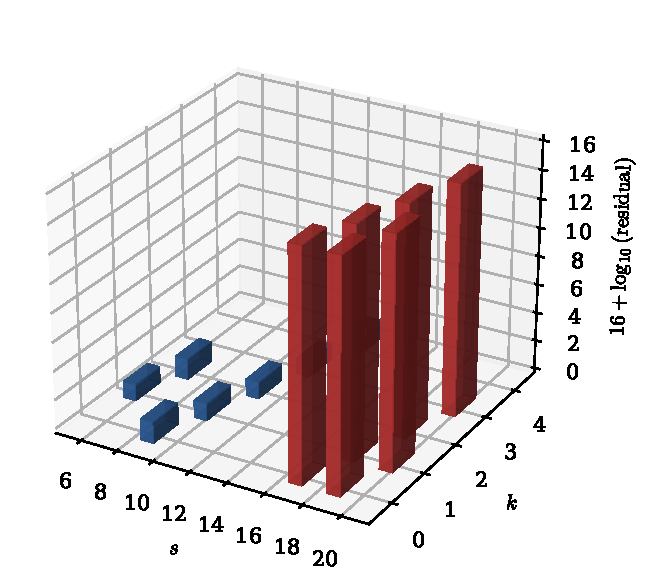
\includegraphics[width=0.66\textwidth]{figures/fig_residuals.pdf}
\caption{Relative residual of the least-squares solution of the absorption equation~\eqref{eq:proj1} for real frames, plotted as $16+\log_{10}(\text{residual})$ against $s$ and $k$. Blue: $(9,1)$, $(10,2)$, $(11,3)$, $(12,4)$, $(13,5)$ with $k=t-1$, and $(6,6)$, $(7,7)$ with $k=1,2$, all with $D'=10$; the residuals are below $3\times10^{-15}$. Red: $(17,1)$, $(18,2)$, $(19,3)$, $(20,4)$ with every tested $k$, $D'\in\{16,18,20,22\}$; the residuals lie between $0.97$ and $1$, so no solution is found in these samples; the exact exclusion follows from the analytic theorem.}
\label{fig:residuals}
\end{figure}

\section{A single time: counting states}
\label{sec:singletime}

For the first family in~\eqref{eq:families} the time is single, and representation theory gives a bound that does not depend on how the theory is constructed. Consider a unitary, Poincaré-invariant quantum theory in $\bR^{9+8n,1}$ with $n\ge1$, whose supercharges $Q_\alpha$ form one Majorana--Weyl spinor, so that there are $S=2^{4+4n}$ real supercharges. By Proposition~\ref{prop:sym2} the most general anticommutator is
\begin{equation}
\label{eq:QQ}
\{Q_\alpha,Q_\beta\}=(\gamma^\mu\mathcal C)_{\alpha\beta}P_\mu+\sum_{p\in\{5,9,\dots,5+4n\}}(\gamma^{\mu_1\cdots\mu_p}\mathcal C)_{\alpha\beta}Z_{\mu_1\cdots\mu_p},
\end{equation}
with $\mathcal C$ the charge conjugation matrix and $Z_{[p]}$ tensor charges, in accordance with the general structure of supersymmetry algebras~\cite{HaagLopuszanskiSohnius1975,vanHoltenVanProeyen1982}. Tensor charges of this kind are carried by extended objects~\cite{deAzcarragaGauntlettIzquierdoTownsend1989}; in ten dimensions the five-form charge is carried by five-branes. We state their absence on the massless multiplet as hypothesis~(H).

\begin{theorem}
\label{thm:singletime}
Assume (H) that the tensor charges vanish on a massless supermultiplet. Then the multiplet has at least $2^{S/4}=2^{2^{2+4n}}$ states for each momentum, half of them bosonic. In particular the theory has no massless vector multiplet: such a multiplet would have $D-2=8+8n$ bosonic states for each generator of the gauge algebra.
\end{theorem}

\begin{proof}
On the multiplet, with momentum $p$, $p^2=0$, $p^0>0$, the anticommutator is $M_{\alpha\beta}=(\slashed{p}\,\mathcal C)_{\alpha\beta}$, a real symmetric matrix, positive semidefinite because the $Q_\alpha$ are Hermitian and the norm is positive. Its rank is $S/2$: choosing a real null frame of rank one with $n_1=p$, Lemma~\ref{lem:fock} shows that $\slashed p$ annihilates exactly the half $K$ of each Weyl module. A supercharge $Q$ in the kernel of $M$ has $\{Q,Q\}=0$, so $\|Q\psi\|^2=0$ and $Q$ vanishes on every state $\psi$ of the multiplet. The remaining $S/2=2^{3+4n}$ combinations, rescaled, satisfy $\{\hat Q_a,\hat Q_b\}=2\delta_{ab}$ and generate a complex Clifford algebra on $2^{3+4n}$ generators, whose irreducible representations have dimension $2^{2^{2+4n}}$ and are split evenly by $(-1)^F$. The multiplet is a direct sum of such representations.
\end{proof}

For $n=0$ the bound is $2^4=16$: the eight bosonic and eight fermionic states of ten-dimensional super Yang--Mills theory. For $n=1$, $D=18$, it is $2^{64}$, against sixteen bosonic and $128$ fermionic states of a vector and a Majorana--Weyl gaugino. Figure~\ref{fig:multiplets} shows the gap for $n\le3$. The argument is the one that bounds the helicity of massless supermultiplets in four dimensions by one for sixteen supercharges and by two for thirty-two~\cite{Nahm1978,Strathdee1987}. To exclude arbitrary multiplicities of vector, spinor and scalar fields, a state count alone is insufficient. The following helicity argument supplies the needed bound.

\begin{lemma}[Helicity span]\label{lem:helicityspan}
Under the hypotheses of Theorem~\ref{thm:singletime}, suppose the massless multiplet has a finite helicity spectrum for a rotation $J$ in a transverse two-plane. If $h_{\min}$ and $h_{\max}$ are its least and greatest helicities, then
\[
 h_{\max}-h_{\min}\ge S/8.
\]
In particular a multiplet containing only scalar, spinor and vector polarizations has $S\le16$, independently of their multiplicities.
\end{lemma}
\begin{proof}
Choose the null momentum in a four-dimensional Lorentzian subspace and let $J$ generate rotations in its transverse two-plane. A transverse spinor has $J$-weights $+\tfrac12$ and $-\tfrac12$ with equal multiplicities. In its occupation basis the first occupation fixes this weight, while the chirality condition fixes only the parity of the remaining occupations; there are equally many choices for the two weights. On the $S/2$ real active supercharges, complexification therefore gives $S/4$ operators of each weight. The positive anticommutator of Theorem~\ref{thm:singletime}, invariant under $J$, pairs the two weights nondegenerately. After normalization the operators may be written $a_i^\dagger,a_i$, $1\le i\le S/4$, with
\[
 \{a_i,a_j^\dagger\}=\delta_{ij},\qquad
 \{a_i,a_j\}=\{a_i^\dagger,a_j^\dagger\}=0,\qquad
 [J,a_i^\dagger]=\tfrac12 a_i^\dagger.
\]
Take a unit vector $\Omega$ of helicity $h_{\min}$. Each $a_i$ lowers helicity by $\tfrac12$, so $a_i\Omega=0$. The canonical anticommutation relations give
\[
 \bigl\|a_1^\dagger\cdots a_{S/4}^\dagger\Omega\bigr\|^2=1.
\]
This nonzero vector has helicity $h_{\min}+S/8$, proving the span bound. A scalar has helicity $0$, a spinor has helicities $\pm\tfrac12$, and a vector has helicities $0,\pm1$ under this rotation. Arbitrary multiplicities of these polarizations still have their spectrum in $[-1,1]$. Thus $S/8\le2$, or $S\le16$.
\end{proof}

For $n\ge1$, $S=2^{4+4n}>16$, so a massless multiplet in this unitary, tensor-charge-free class cannot be assembled from any finite number of those low-spin fields. The mechanism is the familiar helicity bound on extended supersymmetry~\cite{Nahm1978,Strathdee1987}; it is written out here to distinguish it from the separate dimension count.

\begin{figure}[t]
\centering
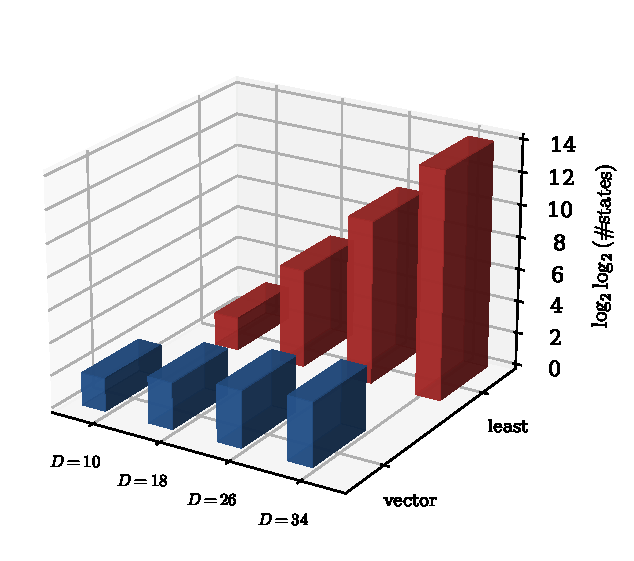
\includegraphics[width=0.66\textwidth]{figures/fig_multiplets.pdf}
\caption{Massless multiplets in $(9+8n)+1$, plotted as $\log_2\log_2$ of the number of states. Blue: a vector field and a Majorana--Weyl gaugino, $(8+8n)+2^{3+4n}$ states. Red: the least number $2^{2^{2+4n}}$ of states of a massless multiplet without tensor charges (Theorem~\ref{thm:singletime}). The two agree only for $D=10$.}
\label{fig:multiplets}
\end{figure}

\section{What this means for \texorpdfstring{$27+3$}{27+3} and \texorpdfstring{$19+3$}{19+3}}
\label{sec:consequences}

In $27+3$ the Weyl spinor has $2^{14}=16\,384$ components, and its symmetric square contains forms of degrees $3$, $7$, $11$ and $15$ only. The anticommutator of two supercharges contains no momentum, and translations can be obtained from it only by contracting a form charge with null vectors, as in~\ref{ax:N4}; this is how all the constructions of Refs.~\cite{NishinoSezgin1996,Sezgin1997,Nishino1998} proceed. With three times $k\le3$, so the residual space has dimension at least $24$, and Corollary~\ref{cor:families} applies: the cubic gaugino terms cannot be absorbed. The same holds in $19+3$, where the residual dimension is at least $16$, and in every other signature of the families~\eqref{eq:families} with $n\ge1$. For any compact non-abelian Lie gauge algebra, the obstruction~\eqref{eq:proj1} already arises on an $\mathfrak{su}(2)$ subalgebra and is unaffected by additional representation labels. A non-Lie extension or other field content would require assumptions beyond the present definition.

The results leave the algebraic structures of Refs.~\cite{RiosMarraniChester2019,TruiniMarraniRios2019,MarraniRiosChester2023} untouched. The superalgebras~(3.5)--(3.8) of Ref.~\cite{RiosMarraniChester2019} exist by Proposition~\ref{prop:sym2}, and so do the cosets and Jordan-algebraic constructions built on them. The obstruction concerns realization by the specific null-projected field theory defined here. Applications invoking a $27+3$ theory by this particular transfer, including a worldvolume theory for M-theory~\cite{RiosMarraniChester2020}, the dark matter model of Ref.~\cite{PaduroiuRiosMarraniChester2021} and the higher M-theories of Ref.~\cite{Banerjee2024}, require a construction outside these five assumptions, or a change to the claimed transfer. Every theory satisfying~(N1)--(N5) obeys the necessary condition $s-t\in\{8,0,-8\}$. For residual dimension greater than two its cubic fermion structure satisfies the ten-dimensional identity. Existence and full dynamics in every remaining signature are separate questions. This agrees with the view, expressed already in Ref.~\cite{RudychevSezginSundell1998}, that the null projections of super Yang--Mills theories beyond ten dimensions encode ten-dimensional theories with a covariant presentation of the extra directions.

Two remarks fix the scope of the results. The Main Theorem concerns theories with a single gaugino of definite chirality and the transformation rules~\ref{ax:N2}. Theories with several gauginos, with new auxiliary fields, or with transformation rules nonlinear in $\lambda$ lie outside it, and are not decided by the Main Theorem. Theorem~\ref{thm:singletime} assumes unitarity and hypothesis~(H), which is why it covers only the single-time family: we do not assume the positive-energy unitary representation used in the counting argument for the several-time signatures. The algebraic Theorem~\ref{thm:main} is the result applied there.

\section{Conclusions}
\label{sec:conclusions}

Supersymmetric Yang--Mills theories built with null projections in signatures with several times are governed by an invariant that the Clifford algebra does not see. The bound $\min(s,t)$ limits the number of null directions that can be projected out of a real gaugino, and a residual dimension greater than two must equal ten because the absorption equation forces the ten-dimensional Fierz identity. The dimension count $N=2(d-2)$ of Theorem~\ref{thm:vector} makes the second statement rigid, and together the two leave only the signatures with $s-t\in\{8,0,-8\}$. The families $(9+8n)+1$, $(10+8n)+2$, $(11+8n)+3$ and $(12+8n)+4$ with $n\ge1$, including $27+3$ and $19+3$, are excluded. For $(9+8n)+1$, Theorem~\ref{thm:singletime} and Lemma~\ref{lem:helicityspan} exclude massless vector multiplets and finite multiplets made only of scalar, spinor and vector fields under the stated unitarity and tensor-charge hypotheses. A supersymmetric gauge theory in these signatures would have to violate the axioms~(N1)--(N5) in an essential way, and it would then no longer be a repetition of Nishino's proof.

\section*{Data availability}

The general results are proved in the text; numerical samples are supplementary. The plotted and tabulated residuals retain the archived reference run. A fresh run of all 34 checks on 24 October 2026 also passed; its output and library versions are included in the submission supplement. This manuscript revision is archived at~\cite{Paper4Revision}. Its complete \LaTeX{} source, numerical programs and verification logs are available in the versioned repository~\cite{Paper4Release}; the earlier source and reference data are archived at~\cite{BhattacharjeeArchive2026}. The schematics of Figs.~\ref{fig:proofmap} and~\ref{fig:cube} are drawn in the \LaTeX{} source with TikZ.

\section*{Use of AI tools}

Claude Code (Anthropic) assisted the original preparation. OpenAI Codex assisted this revision with proof auditing, the explicit helicity-span argument, the null-current lemma, scope corrections and editing. The numerical programs are supplementary checks; they do not certify the general field-theoretic statements. Responsibility for reviewing and approving the final mathematical content rests with the author.

\section*{Funding}

The author received no funding for this work.

\section*{Competing interests}

The author declares no competing interests.

\appendix

\section{The oscillator decomposition}
\label{app:fock}

We prove Lemma~\ref{lem:fock}. The $\Pup_i$ are commuting projections, so the products $\Pi_a=\prod_i\bigl(a_i\Pup_i+(1-a_i)\Pdn_i\bigr)$ are orthogonal idempotents with $\sum_a\Pi_a=1$, and $\Delta=\bigoplus_a\Delta_a$ with $\Delta_a=\Pi_a\Delta$. For $j\ne i$, $\nsl_i$ anticommutes with $\nsl_j$ and $\msl_j$ and therefore commutes with $\Pup_j$. From $\nsl_i^2=0$ and $\nsl_i\msl_i+\msl_i\nsl_i=2$ we get $\nsl_i\msl_i\nsl_i=2\nsl_i$, that is $\Pup_i\nsl_i=\nsl_i$ and $\nsl_i\Pup_i=0$. Hence $\nsl_i$ annihilates $\Delta_a$ when $a_i=1$ and maps $\Delta_a$ into $\Delta_{a+e_i}$ when $a_i=0$; on the latter $\msl_i\nsl_i=2\Pdn_i=2$, so the map is injective. The same argument with $\msl_i$ gives an injection $\Delta_{a+e_i}\to\Delta_a$, so both maps are isomorphisms. This proves (ii), and all the $\Delta_a$ have the same dimension $2^r/2^k$.

Each $\gamma^{\mu'}$ anticommutes with every $b_i$ and $b_i^\dagger$, hence commutes with every $\Pup_i$ and preserves every $\Delta_a$. Therefore $\Delta_a$ is a module over $\Cl(V'_\bC)$, which for even $D'$ is a simple algebra of dimension $2^{2r-2k}$ with a unique irreducible module, of dimension $2^{r-k}$. As $\dim\Delta_a=2^{r-k}$, $\Delta_a$ is that module. This proves (i).

For (iii), Up to the sign $(-1)^{k(k-1)/2}$, $T$ is the composition of the isomorphisms of (ii) along the path $\mathbf 0\to e_1\to e_1+e_2\to\dots\to\mathbf 1$, it annihilates every $\Delta_a$ with $a\ne\mathbf 0$ by (ii), and $\gamma^{\mu'}$ anticommutes with each of its factors. For (iv), by~\eqref{eq:Bsym}, $B(\Pup_i\psi,\chi)=\frac12\theta^2B(\psi,\msl_i\nsl_i\chi)=B(\psi,\Pdn_i\chi)$. So if $\psi\in\Delta_a$, $\chi\in\Delta_b$ and $a_i=b_i=1$, then $B(\psi,\chi)=B(\Pup_i\psi,\chi)=B(\psi,\Pdn_i\chi)=0$, and similarly if $a_i=b_i=0$. For (v), choose an orthonormal basis of $V_\bC$ consisting of a basis of $V'_\bC$ and the vectors $e_i=(n_i+m_i)/\sqrt2$, $f_i=(n_i-m_i)/\sqrt2$, with $e_i^2=1$ and $f_i^2=-1$. Then $\slashed e_i\slashed f_i=\frac12(\msl_i\nsl_i-\nsl_i\msl_i)=\Pdn_i-\Pup_i$, and the chirality operator, proportional to the product of all basis gamma matrices, is $\Gamma_*=\pm\Gamma'_*\prod_i(\Pdn_i-\Pup_i)$, with the sign fixed by $\Gamma_*^2=1$. On $\Delta_a$ the product equals $(-1)^{|a|}$.

\begin{lemma}[Null-frame current]\label{lem:nullcurrent}
Let $\lambda_1,\lambda_2\in K$. After identifying vectors and covectors with the metric, the $(k+1)$-form
\[
 \omega_{\mu_0\cdots\mu_k}
   =B(\lambda_1,\gamma_{\mu_0\cdots\mu_k}\lambda_2)
\]
has the form $v\wedge j$ for a residual one-form $j\in(V')^*_{\bC}$.
\end{lemma}
\begin{proof}
Evaluate $\omega$ on the null-frame basis $n_i,m_i$ and a basis of $V'$. Both spinors are in the fully occupied corner. By Lemma~\ref{lem:fock}(iv), a Clifford word pairing nontrivially with the first spinor must take the second to the empty corner. It must therefore contain every lowering operator $\msl_i$. A word of degree $k+1$ can do this only by using exactly these $k$ operators and one residual generator: an additional raising operator would require another lowering operator and hence at least $k+2$ factors. Antisymmetrization preserves this occupancy count. Thus a nonzero component has one argument $m_i$ for every $i$ and one residual argument. Since $n_i\cdot m_j=\delta_{ij}$, these are exactly the components of $v\wedge j$.
\end{proof}

\section{Numerical checks in explicit gamma matrices}
\label{app:checks}

The program \texttt{verify.py} in the repository builds the gamma matrices of $\bR^{s,t}$ as Kronecker products of Pauli matrices, multiplying the first $t$ Euclidean generators by $i$, and checks the Clifford relations. It finds a charge conjugation matrix $\mathcal C$ with $\mathcal C\gamma^\mu\mathcal C^{-1}=\pm(\gamma^\mu)^T$ among the products of the real or of the imaginary Euclidean generators, and builds the vector forms of Definition~\ref{def:vector} from it. It then runs the following checks, all of which pass (34 checks, no failures; runtime depends on the numerical libraries and hardware).
\begin{enumerate}[label=(\alph*)]
\item Proposition~\ref{prop:sym2}: the dimension count for $r=2,\dots,20$, and the form degrees of the four families~\eqref{eq:families} for $n=0,1,2$.
\item The identity~\eqref{eq:star} on random spinors: it holds in $(9,1)$, $(5,5)$ and $(1,9)$ (relative residual at most $1.3\times10^{-16}$) and fails in $(17,1)$, $(13,5)$, $(9,9)$ and $(25,1)$ (relative residual between $0.09$ and $0.36$).
\item The identity~\eqref{eq:R} with $j$ fitted by least squares: $j=-0.5000$ in $(9,1)$ and $(5,5)$; no $j$ fits in $(17,1)$ and $(25,1)$ (residual at least $0.99$).
\item Lemma~\ref{lem:traces}(b),(c) in $(9,1)$ and $(17,1)$, exactly.
\item The absorption equation~\eqref{eq:proj1}, solved by least squares for $J$ over random $\lambda\in K$ and $\epsilon\in\Khat$ with explicit real frames $\nsl_i=(\gamma_{\text{space}}+\gamma_{\text{time}})/\sqrt2$; see Table~\ref{tab:absorb} and Fig.~\ref{fig:residuals}.
\item Lemma~\ref{lem:reality} in $(17,1)$ with a complex frame of rank four: the complex conjugate of each $n_i$ is $m_i$, and $\nsl_i\msl_i+\msl_i\nsl_i=2$, so the occupied corner contains no Majorana spinor.
\item Lemma~\ref{lem:witt}: real null frames of rank $\min(s,t)$ satisfying~\eqref{eq:frame}.
\item Theorem~\ref{thm:singletime}: the counts of Fig.~\ref{fig:multiplets} for $n=0,1,2,3$.
\end{enumerate}

\begin{table}[htbp]
\centering
\begin{adjustbox}{max width=\linewidth,max totalheight=.80\textheight}\begin{tabular}{@{}ccccccc@{}}
\toprule
$(s,t)$ & $k$ & frame & $D'$ & $\dim K_\chi$ & residual & solvable \\
\midrule
$(9,1)$ & 0 & -- & 10 & 16 & $3.0\times10^{-15}$ & yes\\
$(10,2)$ & 1 & real & 10 & 16 & $1.6\times10^{-15}$ & yes\\
$(11,3)$ & 2 & real & 10 & 16 & $1.5\times10^{-15}$ & yes\\
$(12,4)$ & 3 & real & 10 & 16 & $1.4\times10^{-15}$ & yes\\
$(13,5)$ & 4 & real & 10 & 16 & $2.6\times10^{-15}$ & yes\\
$(6,6)$ & 1 & real & 10 & 16 & $1.4\times10^{-15}$ & yes\\
$(7,7)$ & 2 & real & 10 & 16 & $2.8\times10^{-15}$ & yes\\
$(17,1)$ & 0 & -- & 18 & 256 & $0.98$ & no\\
$(18,2)$ & 1 & real & 18 & 256 & $0.99$ & no\\
$(19,3)$ & 0 & -- & 22 & 1024 & $1.0$ & no\\
$(19,3)$ & 2 & real & 18 & 256 & $0.99$ & no\\
$(20,4)$ & 1 & real & 22 & 1024 & $1.0$ & no\\
$(20,4)$ & 3 & real & 18 & 256 & $0.98$ & no\\
$(17,1)$ & 4 & complex & 10 & 16 & $1.7\times10^{-15}$ & yes (complex sector)\\
$(19,3)$ & 2 & complex & 18 & 256 & $0.97$ & no\\
\bottomrule
\end{tabular}\end{adjustbox}
\caption{The absorption equation~\eqref{eq:proj1} in explicit gamma matrices. The residual is the relative norm of the least-squares remainder over three random draws. These samples are consistent with the analytic obstruction of Theorem~\ref{thm:reduction} for $D'>2$; the complex frame in $(17,1)$ is the case of Remark~\ref{rem:complex}.}
\label{tab:absorb}
\end{table}

\section{Symmetric squares for the four families}
\label{app:tables}

Table~\ref{tab:sym2} lists $\Sym^2\Delta_+$, by Proposition~\ref{prop:sym2}, for the families~\eqref{eq:families} with $n=0,1,2$, together with the residual dimension $s-t$ of a real null frame of the largest rank $k=t$. The momentum $\Lambda^1$ occurs only in the first family. Since $D'$ decreases as $k$ grows, a residual dimension of ten is reachable only when $s-t\le10$, that is only for $n=0$.

\begin{table}[htbp]
\centering
\begin{adjustbox}{max width=\linewidth,max totalheight=.80\textheight}\begin{tabular}{@{}cccccc@{}}
\toprule
$(s,t)$ & $D$ & $\dim\Delta_+$ & degrees in $\Sym^2\Delta_+$ & $\dim\Sym^2\Delta_+$ & $D'$ at $k=t$ \\
\midrule
$(9,1)$ & 10 & 16 & 5, 1 & 136 & 8\\
$(10,2)$ & 12 & 32 & 6, 2 & 528 & 8\\
$(11,3)$ & 14 & 64 & 7, 3 & 2\,080 & 8\\
$(12,4)$ & 16 & 128 & 8, 4, 0 & 8\,256 & 8\\
\midrule
$(17,1)$ & 18 & 256 & 9, 5, 1 & 32\,896 & 16\\
$(18,2)$ & 20 & 512 & 10, 6, 2 & 131\,328 & 16\\
$(19,3)$ & 22 & 1\,024 & 11, 7, 3 & 524\,800 & 16\\
$(20,4)$ & 24 & 2\,048 & 12, 8, 4, 0 & 2\,098\,176 & 16\\
\midrule
$(25,1)$ & 26 & 4\,096 & 13, 9, 5, 1 & 8\,390\,656 & 24\\
$(26,2)$ & 28 & 8\,192 & 14, 10, 6, 2 & 33\,558\,528 & 24\\
$(27,3)$ & 30 & 16\,384 & 15, 11, 7, 3 & 134\,225\,920 & 24\\
$(28,4)$ & 32 & 32\,768 & 16, 12, 8, 4, 0 & 536\,887\,296 & 24\\
\bottomrule
\end{tabular}\end{adjustbox}
\caption{Symmetric squares of the Weyl spinor for the families~\eqref{eq:families}, $n=0,1,2$. The last column is $s-t=s+t-2\min(s,t)$, the residual dimension of a real null frame of rank $k=t$. For $n=0$ Nishino's frames have $k=t-1$ and $D'=10$; a frame with $k=t$ gives $D'=8$, which Theorem~\ref{thm:reduction} excludes. For $n\ge1$ every admissible frame has $D'\ge16$.}
\label{tab:sym2}
\end{table}

\FloatBarrier

\begin{thebibliography}{99}

\bibitem{BrinkSchwarzScherk1977}
L.~Brink, J.~H.~Schwarz and J.~Scherk, \textit{Supersymmetric Yang--Mills theories}, Nucl.\ Phys.\ B \textbf{121} (1977) 77, \doilink{10.1016/0550-3213(77)90328-5}.

\bibitem{KugoTownsend1983}
T.~Kugo and P.~K.~Townsend, \textit{Supersymmetry and the division algebras}, Nucl.\ Phys.\ B \textbf{221} (1983) 357, \doilink{10.1016/0550-3213(83)90584-9}.

\bibitem{Evans1988}
J.~M.~Evans, \textit{Supersymmetric Yang--Mills theories and division algebras}, Nucl.\ Phys.\ B \textbf{298} (1988) 92, \doilink{10.1016/0550-3213(88)90305-7}.

\bibitem{BaezHuerta2010}
J.~C.~Baez and J.~Huerta, \textit{Division algebras and supersymmetry I}, in \textit{Superstrings, Geometry, Topology, and $C^*$-algebras}, Proc.\ Sympos.\ Pure Math.\ \textbf{81}, American Mathematical Society, Providence (2010), p.~65, \doilink{10.1090/pspum/081/2681758}, \arxiv{0909.0551}.

\bibitem{GreenSchwarz1984}
M.~B.~Green and J.~H.~Schwarz, \textit{Covariant description of superstrings}, Phys.\ Lett.\ B \textbf{136} (1984) 367, \doilink{10.1016/0370-2693(84)92021-5}.

\bibitem{AchucarroEvansTownsendWiltshire1987}
A.~Ach\'ucarro, J.~M.~Evans, P.~K.~Townsend and D.~L.~Wiltshire, \textit{Super $p$-branes}, Phys.\ Lett.\ B \textbf{198} (1987) 441, \doilink{10.1016/0370-2693(87)90896-3}.

\bibitem{BergshoeffSezginTownsend1987}
E.~Bergshoeff, E.~Sezgin and P.~K.~Townsend, \textit{Supermembranes and eleven-dimensional supergravity}, Phys.\ Lett.\ B \textbf{189} (1987) 75, \doilink{10.1016/0370-2693(87)91272-X}.

\bibitem{BlencoweDuff1988}
M.~P.~Blencowe and M.~J.~Duff, \textit{Supermembranes and the signature of space-time}, Nucl.\ Phys.\ B \textbf{310} (1988) 387, \doilink{10.1016/0550-3213(88)90155-1}.

\bibitem{Vafa1996}
C.~Vafa, \textit{Evidence for F-theory}, Nucl.\ Phys.\ B \textbf{469} (1996) 403, \doilink{10.1016/0550-3213(96)00172-1}, \arxiv{hep-th/9602022}.

\bibitem{Bars1997}
I.~Bars, \textit{S-theory}, Phys.\ Rev.\ D \textbf{55} (1997) 2373, \doilink{10.1103/PhysRevD.55.2373}, \arxiv{hep-th/9607112}.

\bibitem{Bars1997b}
I.~Bars, \textit{A case for 14 dimensions}, Phys.\ Lett.\ B \textbf{403} (1997) 257, \doilink{10.1016/S0370-2693(97)00550-9}, \arxiv{hep-th/9704054}.

\bibitem{BarsKounnas1997}
I.~Bars and C.~Kounnas, \textit{Theories with two times}, Phys.\ Lett.\ B \textbf{402} (1997) 25, \doilink{10.1016/S0370-2693(97)00452-8}, \arxiv{hep-th/9703060}.

\bibitem{BarsDelidumanAndreev1998}
I.~Bars, C.~Deliduman and O.~Andreev, \textit{Gauged duality, conformal symmetry and spacetime with two times}, Phys.\ Rev.\ D \textbf{58} (1998) 066004, \doilink{10.1103/PhysRevD.58.066004}, \arxiv{hep-th/9803188}.

\bibitem{Bars2000}
I.~Bars, \textit{Two-time physics in field theory}, Phys.\ Rev.\ D \textbf{62} (2000) 046007, \doilink{10.1103/PhysRevD.62.046007}, \arxiv{hep-th/0003100}.

\bibitem{Hull1998}
C.~M.~Hull, \textit{Duality and the signature of space-time}, JHEP \textbf{11} (1998) 017, \doilink{10.1088/1126-6708/1998/11/017}, \arxiv{hep-th/9807127}.

\bibitem{Hull1998b}
C.~M.~Hull, \textit{Timelike T-duality, de Sitter space, large $N$ gauge theories and topological field theory}, JHEP \textbf{07} (1998) 021, \doilink{10.1088/1126-6708/1998/07/021}, \arxiv{hep-th/9806146}.

\bibitem{RudychevSezgin1997}
I.~Rudychev and E.~Sezgin, \textit{Superparticles in $D>11$}, Phys.\ Lett.\ B \textbf{415} (1997) 363, \doilink{10.1016/S0370-2693(97)01307-5}, \arxiv{hep-th/9704057}.

\bibitem{Nishino1998b}
H.~Nishino, \textit{Supergravity in $10+2$ dimensions as consistent background for superstring}, Phys.\ Lett.\ B \textbf{428} (1998) 85, \doilink{10.1016/S0370-2693(98)00374-8}, \arxiv{hep-th/9703214}.

\bibitem{NishinoSezgin1996}
H.~Nishino and E.~Sezgin, \textit{Supersymmetric Yang--Mills equations in $10+2$ dimensions}, Phys.\ Lett.\ B \textbf{388} (1996) 569, \doilink{10.1016/S0370-2693(96)01181-1}, \arxiv{hep-th/9607185}.

\bibitem{Sezgin1997}
E.~Sezgin, \textit{Super Yang--Mills in $(11,3)$ dimensions}, Phys.\ Lett.\ B \textbf{403} (1997) 265, \doilink{10.1016/S0370-2693(97)00516-9}, \arxiv{hep-th/9703123}.

\bibitem{RudychevSezginSundell1998}
I.~Rudychev, E.~Sezgin and P.~Sundell, \textit{Supersymmetry in dimensions beyond eleven}, Nucl.\ Phys.\ B Proc.\ Suppl.\ \textbf{68} (1998) 285, \doilink{10.1016/S0920-5632(98)00162-5}, \arxiv{hep-th/9711127}.

\bibitem{Nishino1998}
H.~Nishino, \textit{Supersymmetric Yang--Mills theories in $D\ge12$}, Nucl.\ Phys.\ B \textbf{523} (1998) 450, \doilink{10.1016/S0550-3213(98)00113-8}, \arxiv{hep-th/9708064}.

\bibitem{RiosMarraniChester2019}
M.~Rios, A.~Marrani and D.~Chester, \textit{Geometry of exceptional super Yang--Mills theories}, Phys.\ Rev.\ D \textbf{99} (2019) 046004, \doilink{10.1103/PhysRevD.99.046004}, \arxiv{1811.06101}.

\bibitem{RiosMarraniChester2020}
M.~Rios, A.~Marrani and D.~Chester, \textit{Exceptional super Yang--Mills in $27+3$ and worldvolume M-theory}, Phys.\ Lett.\ B \textbf{808} (2020) 135674, \doilink{10.1016/j.physletb.2020.135674}, \arxiv{1906.10709}.

\bibitem{PaduroiuRiosMarraniChester2021}
S.~Paduroiu, M.~Rios, A.~Marrani and D.~Chester, \textit{Warm dark matter from higher-dimensional gauge theories}, Universe \textbf{7} (2021) 462, \doilink{10.3390/universe7120462}, \arxiv{2202.08459}.

\bibitem{MarraniRiosChester2023}
A.~Marrani, M.~Rios and D.~Chester, \textit{Monstrous M-theory}, Symmetry \textbf{15} (2023) 490, \doilink{10.3390/sym15020490}, \arxiv{2008.06742}.

\bibitem{TruiniMarraniRios2019}
P.~Truini, A.~Marrani and M.~Rios, \textit{Exceptional periodicity and magic star algebras. I: Foundations}, \arxiv{1909.00357}.

\bibitem{Banerjee2024}
P.~Banerjee, \textit{Worldvolume origin of higher M theories}, \arxiv{2401.13706}.

\bibitem{Deligne1999}
P.~Deligne, \textit{Notes on spinors}, in \textit{Quantum Fields and Strings: A Course for Mathematicians}, vol.~1, American Mathematical Society, Providence (1999), pp.~99--135.

\bibitem{VanProeyen1999}
A.~Van Proeyen, \textit{Tools for supersymmetry}, Ann.\ Univ.\ Craiova Phys.\ \textbf{9} (1999) 1, \arxiv{hep-th/9910030}.

\bibitem{DAuriaFerraraLledoVaradarajan2001}
R.~D'Auria, S.~Ferrara, M.~A.~Lled\'o and V.~S.~Varadarajan, \textit{Spinor algebras}, J.\ Geom.\ Phys.\ \textbf{40} (2001) 101, \doilink{10.1016/S0393-0440(01)00023-7}, \arxiv{hep-th/0010124}.

\bibitem{LawsonMichelsohn1989}
H.~B.~Lawson and M.-L.~Michelsohn, \textit{Spin Geometry}, Princeton University Press, Princeton (1989).

\bibitem{vanHoltenVanProeyen1982}
J.~W.~van Holten and A.~Van Proeyen, \textit{$N=1$ supersymmetry algebras in $d=2,3,4$ mod $8$}, J.\ Phys.\ A \textbf{15} (1982) 3763, \doilink{10.1088/0305-4470/15/12/028}.

\bibitem{Witt1937}
E.~Witt, \textit{Theorie der quadratischen Formen in beliebigen K\"orpern}, J.\ Reine Angew.\ Math.\ \textbf{176} (1937) 31, \doilink{10.1515/crll.1937.176.31}.

\bibitem{Lam2005}
T.~Y.~Lam, \textit{Introduction to Quadratic Forms over Fields}, Grad.\ Stud.\ Math.\ \textbf{67}, American Mathematical Society, Providence (2005), \doilink{10.1090/gsm/067}.

\bibitem{FreedmanVanProeyen2012}
D.~Z.~Freedman and A.~Van Proeyen, \textit{Supergravity}, Cambridge University Press, Cambridge (2012), \doilink{10.1017/CBO9781139026833}.

\bibitem{HaagLopuszanskiSohnius1975}
R.~Haag, J.~T.~{\L}opusza\'nski and M.~Sohnius, \textit{All possible generators of supersymmetries of the S-matrix}, Nucl.\ Phys.\ B \textbf{88} (1975) 257, \doilink{10.1016/0550-3213(75)90279-5}.

\bibitem{deAzcarragaGauntlettIzquierdoTownsend1989}
J.~A.~de~Azc\'arraga, J.~P.~Gauntlett, J.~M.~Izquierdo and P.~K.~Townsend, \textit{Topological extensions of the supersymmetry algebra for extended objects}, Phys.\ Rev.\ Lett.\ \textbf{63} (1989) 2443, \doilink{10.1103/PhysRevLett.63.2443}.

\bibitem{Nahm1978}
W.~Nahm, \textit{Supersymmetries and their representations}, Nucl.\ Phys.\ B \textbf{135} (1978) 149, \doilink{10.1016/0550-3213(78)90218-3}.

\bibitem{Strathdee1987}
J.~A.~Strathdee, \textit{Extended Poincar\'e supersymmetry}, Int.\ J.\ Mod.\ Phys.\ A \textbf{2} (1987) 273, \doilink{10.1142/S0217751X87000120}.

\bibitem{Paper4Revision}
D. Bhattacharjee, \emph{Residual-dimension obstructions for null-projected
supersymmetric Yang--Mills theories}, Zenodo, version 1.1.0 (2026),
\href{https://doi.org/10.5281/zenodo.23611588}{10.5281/zenodo.23611588}.

\bibitem{Paper4Release}
D. Bhattacharjee, \emph{Source and verification files for residual-dimension
obstructions for null-projected supersymmetric Yang--Mills theories},
version 1.1.0 (2026),
\href{https://github.com/creelie/Paper_4/tree/v1.1.0}{github.com/creelie/Paper\_4, tag v1.1.0}.

\bibitem{BhattacharjeeArchive2026}
D.~Bhattacharjee, \textit{Supersymmetric Yang--Mills theories with several times reduce to ten dimensions: paper and verification code}, version 1.0.0, Zenodo (2026), \doilink{10.5281/zenodo.23558751}.

\end{thebibliography}

\end{document}
